\DontNumberThisInToc
\DontFrameThisInToc
\glsresetall
\ChapterNumberCitation{Cadre de mod\'elisation: Les r\'eseaux de neurones dynamiques}{Whatever exists at all exists in some amount.}{E.L. Thorndike.}{10cm}
\Citation{L'identité entre états mentaux et états physiologiques ou physico-chimiques du cerveau s'impose en toute légitimité... Toute
activité mentale quelle qu'elle soit, réflexion ou décision, émotion ou sentiment, conscience
de soi... est déterminée par l'ensemble des influx nerveux circulant sur des ensembles définis
de cellules nerveuses... J'irais même plus loin en disant qu'elle n'est que cela".}{Changeux Jean-Pierre.L'Homme neuronal (1983). }{10cm}


\section{Introduction}

En biologie, comme dans plusieurs autres domaines, les systèmes dynamiques sont décrits par des équations différentielles qui représentent la variation dans le temps et$/$ou dans l'espace des échanges de matière, d'énergie, d'information ou d'autres quantités. La théorie nous enseigne qu'une solution existe au problème de Cauchy\footnote{\'Etant donnés un intervalle ouvert $U$ de $\mathbf{R} X \mathbf{R}^m$ et une fonction continue f: $U\rightarrow\mathbf{R}^m$, on considère l'équation différentielle (E) : $y' = f (t, y); (t, y) \in U; t \in R; y \in \mathbf{R}^m$. Étant donné un point $(t_0,y_0) \in U$, les entrées sont pondérées par des coefficients (\textit{poids}) approchant les caractéristiques des synapses (fig\ref{Albin}).\\  Le problème de Cauchy consiste à trouver une solution y : $I\rightarrow\mathbf{R}^m$ de (E)  sur un intervalle $I$ contenant $t_0$ dans son intérieur, telle que $y(t_0) = y_0$.} correspondant, mais la pratique nous apprend qu'il n'est parfois pas possible d'expliciter cette solution analytiquement d'o\`u le recours aux solutions approchées numériquement.\\

C'est le cas pour le \textit{neurone biologique} (ou cellule nerveuse) \footnote{Voir \cite{Kandel:1985} pour une introduction à la neuroscience} qui est un système dynamique composé principalement de trois parties (fig \ref{neurone}): le corps cellulaire (le soma), l'axone et les dendrites. Les zones de contact entre un neurone et un autre, ou entre un neurone et une autre cellule s'appellent les synapses. Selon les types de modèles, les niveaux de détail de ces parties ainsi que les mécanismes qui les régissent diffèrent. Dans notre approche, nous avons choisi des modèles simples de la cellule neuronale tout en gardant quelques propriétés importantes, afin de pouvoir simuler des populations de plusieurs unités et ne pas rester à l'échelle du neurone lui-même. De nombreux modèles de neurones sont régis par des équations différentielles qui sont en général très complexes surtout lorsqu'on cherche à faire des modèles biophysiques bien précis.\\

Il est donc nécessaire de s'intéresser à l'étude de simplifications qui permettent tout de même de capturer les propriétés essentielles du calcul neuronal, dans le cadre des fonctions que l'on cherche à réaliser. Mais ceci n'est pas facile vu la nature du système étudié. En effet, le système est bouclé et les neurones communiquent entre eux. En outre, le système est distribué donc chaque neurone doit être considéré comme un processeur élémentaire, son calcul devant être rapide. De plus, de nombreux paramètres et constantes de temps peuvent agir sur la stabilité du système (les attracteurs, les points fixes, les cycles, etc.).\\

En résumé, même si l'équation qui gouverne le neurone élémentaire est simplifiée, une étude purement analytique ne permet généralement pas de conna\^itre les propriétés d'un système neuronal et le recours à des simulations est indispensable pour étudier empiriquement les caractéristiques obtenues par le choix d'un certain schéma de calcul. Il est aussi important d'établir des schémas de calculs numériques permettant de transformer ces équations différentielles continues en calculs discrets en temps et en espace pour pouvoir calculer itérativement les évolutions des états des neurones.\\%

En outre, les réseaux de neurones artificiels sont souvent considérés comme des architectures distribuées, où de nombreux éléments de traitement simples fonctionnent en parallèle. Cela a été clairement introduit dans le travail de \cite {Rumelhart:1987}, qui a souligné la nature parallèle du traitement neuronal. Cependant, aucun des huit principes de calcul proposés ne souligne la notion de \textit{synchronisation} dans le traitement neuronal. En effet, il est implicitement supposé que le calcul est \textit{synchrone}, et c'est le cas dans la plupart des réseaux de neurones artificiels d'aujourd'hui. Cette position est contestable d'un point de vue neurobiologique puisque le cerveau est considéré comme un système oscillant dynamique régulièrement perturbé par les variations externes (l'environnement, les stimuli, etc) et/ou les événements internes (décharges, hormones, rythme cardiaque, etc.). Il ne repose pas sur une horloge centrale qui donnerait un signal général à toutes les unités du système pour se mettre à jour simultanément. Cependant, l'absence de cette horloge centrale ne devrait pas empêcher, ni la synchronisation de se produire entre les neurones, ni la rythmicité (comme les oscillations thêta rythmiques provenant de la région septale).\\ 

Nous proposons dans ce chapitre d'étudier les caractéristiques du calcul neuronal. Plus précisément, nous allons décrire la structure et le fonctionnement de l'unité de base : le neurone ({\em calcul local}). Ensuite, nous allons introduire la théorie des champs de neurones dynamiques [\gls{dnf}] qui offre un cadre de calcul intéressant pour la modélisation des phénomènes corticaux. Puis, nous aborderons brièvement la notion de plasticité synaptique ({\em calcul adaptatif}). Enfin, dans le cadre de cette thèse, nous nous sommes intéressés, en particulier, à deux aspects importants de la modélisation des DNF, à savoir l'intégration numérique et les problèmes de discrétisation d'une part ({\em calcul discret}), et l'évaluation et les problèmes de synchronisation temporelle d'autre part ({\em calcul distribué}). Nous ne cherchons pas à donner un état de l'art complet sur ces questions, mais plutôt à montrer comment un concept général, appelé ici {\em paradigme totalement asynchrone}, peut fournir une réponse satisfaisante en se basant sur des résultats connus des systèmes discrets asynchrones et en les reliant au domaine des neurosciences computationnelles.\\

%%%%%%%%%%%%%%%%%%%%%%%%%%%%%%%%%%%%%%%%%%%%%%%%%%%%%%%%%%%%%%%%%%%%%%%%%%%%%%%%%%%%%%%%%%%%%%
\section{Qu'est ce qu'un neurone: une règle locale}

 Nous allons présenter dans cette partie les caractéristiques de cette unité de base du système nerveux en partant de la biologie pour arriver à la modélisation (le neurone artificiel).

\subsection{Le neurone biologique}

Le neurone est décrit classiquement comme l'enchaînement de quatre fonctions. Les dendrites assurent la réception de l'influx nerveux envoyé par les autres neurones (fig \ref{neurone}). Le corps cellulaire analyse et intègre l'information reçue. Cette information est traitée et le signal de sortie est renvoyé à travers l'axone. Les synapses assurent la connexion entre les neurones via des mécanismes chimiques d'échange de \textit{neurotransmetteurs} entre les ramifications des dendrites et les terminaisons des axones des autres neurones. Le fonctionnement du neurone est assuré principalement par la variation de son \textit{potentiel de membrane}.\\ %L'axone transmet l'information traitée sous forme de \textit{spikes}

\begin{figure}[htbp]
\begin{center}
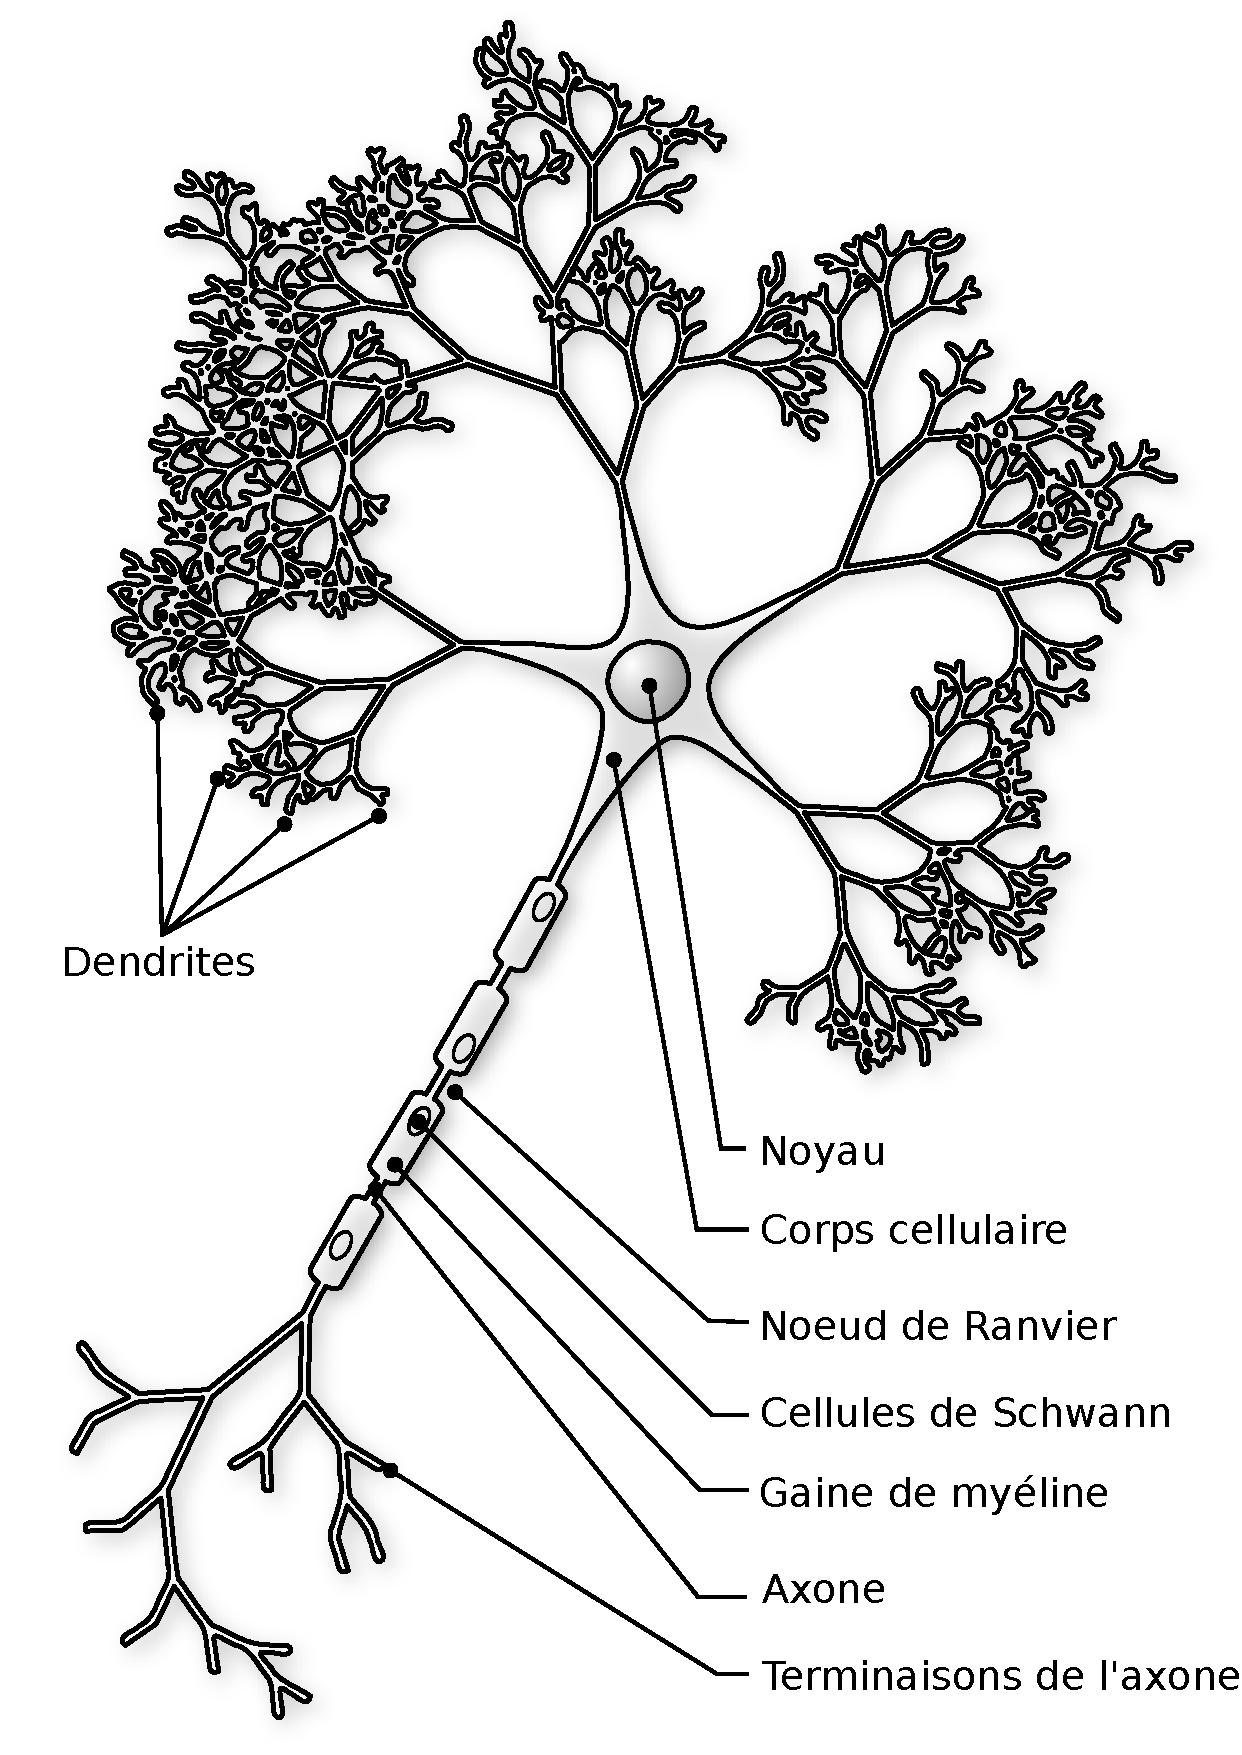
\includegraphics[height=0.5\textwidth]{figures/ch1_1_neurone}
\end{center}
\caption{Schéma d'un neurone biologique [wikipedia]}
\label{neurone}
\end{figure}

En effet, les membranes cellulaires en général, et les membranes des cellules nerveuses, en particulier, maintiennent une faible tension ou «potentiel» dans leur état normal de repos. Ce potentiel membranaire provient d'une différence de concentrations (entre l'extérieur et l'intérieur de la membrane) en électrolytes de calcium ($Ca^{2+}$), potassium ($K^{+}$) et sodium ($Na^{+}$). Un neurone est donc caractérisé par un potentiel de repos qui vaut généralement $-65mV$ mais qui peut varier selon le type de neurone considéré \cite{Kandel:2000}. Cette polarisation est assurée par l'action de canaux-ioniques voltage-dépendants qui régulent la concentration des ions. Quand le potentiel de membrane dépasse la valeur de repos, on parle de \textit{dépolarisation} et dans le cas contraire, on parle d'\textit{hyperpolarisation}. \\

Les variations du potentiel membranaire induisent de courtes impulsions électriques dont l'amplitude est d'environ $100mV$ et dont la durée moyenne est d'une milliseconde (fig \ref{potentiel}). Ces impulsions, appelées \textit{spikes} (pointes) ou \textit{potentiels d'action}, sont capables de se propager le long des axones permettant ainsi la transmission des informations. Nous aborderons dans la suite la question du codage neuronal. \\

\begin{figure}[htbp]
\begin{center}
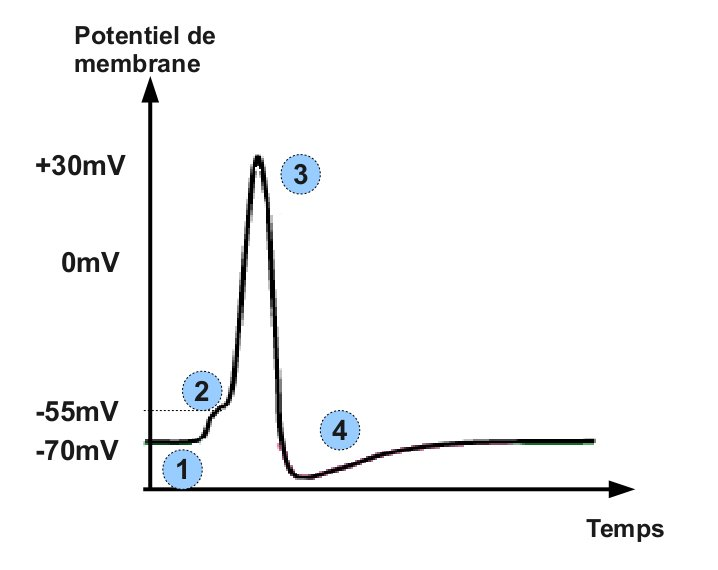
\includegraphics[width=0.4\textwidth]{figures/ch1_2_potentiel}
\end{center}
\caption{Les différentes phases du potentiel d'action. 1: prépotentiel, phase de repos. 2: dépolarisation de la membrane. 3: repolarisation rapide. 4: période réfractaire, hyperpolarisation.}
\label{potentiel}
\end{figure}

Les spikes sont des évènements discrets stéréotypés qui peuvent se produire à des intervalles réguliers ou pas. Ils se propagent le long de l'axone sans modifications. Une suite de potentiels est appelée \textit{train de spikes}. Ils sont généralement bien séparés, puisque un neurone passe par une \textit{période réfractaire} après l'émission d'un spike pendant laquelle il est silencieux (pas de spikes émis). \\

En effet, quand un spike arrive à une synapse à partir d'un neurone activé (neurone pré-synaptique), une substance chimique appelée neurotransmetteur est libérée provoquant l'ouverture des canaux ioniques dans la membrane du neurone au repos (neurone post-synaptique). Les ions circulent donc à travers les canaux créant un changement dans la polarisation membranaire de repos. Une variation temporaire dans la polarisation électrique de la membrane d'un neurone est appelée \textit{potentiel post-synaptique} [\gls{psp}]. Il s'agit d'un signal de réponse rapide très faible qui se déplace à travers la membrane et qui s'affaiblit en s'éloignant de son site de production. L'accumulation de \glspl{psp} reçus peut agir sur la probabilité d'émission de spikes, en particulier, quand la dépolarisation résultante est assez forte, le neurone se décharge: il émet un spike. Les \glspl{psp} sont appelés excitateurs (EPSP) s'ils augmentent la probabilité qu'un potentiel d'action post-synaptique se produise et inhibiteur (IPSP) s'ils diminuent cette probabilité.\\

La communication entre les neurones est assurée donc par ces transmissions de potentiels d'action. Leur génération fonctionne sur le mode ``tout ou rien'' puisqu'un spike ne peut être émis que si le seuil d'excitation du neurone est atteint. \\



En résumé, l'activité électrique des neurones est complexe. La communication entre eux est assurée par la transmission de potentiels d'action. Enfin, puisque les spikes sont d'amplitude et d'intensité invariables, un potentiel d'action isolé ne comporte qu'une petite partie de l'information. C'est plutôt le nombre et le timing de l'ensemble des spikes émis qui portent la majorité de l'information à traiter. Donc c'est la séquence de spikes émis qui contient le message transmis d'un neurone à un autre mais la question est de savoir quel est le code utilisé par les neurones pour traiter ce flux d'informations binaires?  \\  

%%%%%%%%%%%%%%%%%%%%%%%%%%%%%%%%%%%%%%%%%%%%%%%%%%%%%%%%%%%%%%%%%%%%%%%%%%%%%%%%%%%%%%%%%%%%%%%%%%%%%%%%%%%%%%%%%%%%%%%%%%%%%%%%%%%%%%%%%%%%%%%%%%%%%%%%%%%%%%%%%%%%%%%%%%%%%%%%%%%%%%%%%%%%%%%%%%%%
\subsection{Qu'est ce qui code l'information?}

Plusieurs expérimentalistes et théoriciens se sont intéressés à la question de savoir comment lire les trains de spikes (\ref{train}) pour comprendre la communication neuronale. Plusieurs propositions existent \cite{Shadlen:1994, Rieke:1996, Borst:1999,  Gerstner:2002, Pouget:2003, Averbeck:2004, Cariani:2004}.\\


\begin{figure}[htbp]
\begin{center}
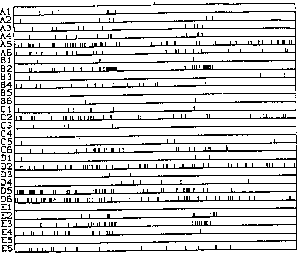
\includegraphics[width=0.4\textwidth]{figures/ch1_3_train}
\end{center}
\caption{Exemple d'enregistrement de trains de spikes de 30 neurones. Chaque ligne correspond à un neurone. L'axe horizontal représente le temps (en total 4000ms). Chaque impulsion est représentée par un petit trait vertical (Kruger et Aiple, 1988)}
\label{train}
\end{figure}

La question que l'on se pose porte sur l'information contenue dans une telle représentation spatio-temporelle des spikes: quel est le code utilisé pour transmettre ces signaux et quel est le mécanisme utilisé par les autres neurones pour les décoder ?\\

Deux stratégies de codage sont généralement décrites. La première stratégie est le codage \textit{fréquentiel} qui consiste à compter les spikes et les moyenner par rapport au temps, par rapport aux essais expérimentaux ou par rapport aux populations de neurones pour déterminer un niveau d'activité. Plusieurs études supposent que la plupart de l'information est contenue dans \textit{la fréquence moyenne de décharge} qui est devenue un outil standard pour décrire les propriétés des neurones sensoriels ou corticaux \cite{Mountcastle:1957, Hubel:1959}. Cependant, une telle hypothèse néglige l'information contenue dans les dates d'occurences individuelles des spikes \cite{Oram:1999, Abeles:1994, Hopfield:1995, Bialek:1991, Shadlen:1994, Rieke:1996}. La seconde stratégie de codage, dite \textit{impulsionnelle}, repose sur le profil temporel de la séquence de spikes. Elle permet de conserver l'information temporelle concernant les impulsions individuelles, sur une échelle de temps d'une milliseconde \cite{Rieke:1997}. Nous passerons d'abord en revue certaines méthodes de codage impulsionnel. Ensuite nous nous concentrerons sur le codage fréquentiel. 


\subsubsection{Codage impulsionnel}
Nous allons présenter ici trois stratégies possibles du codage impulsionnel (codage à spikes): 
\paragraph{Les premiers spikes décident:}

\cite{Thorpe:1996} propose que la rapidité de la réponse dans des tâches de discrimination visuelle implique que la décision se fait dès les tous premiers spikes. Il fait valoir que le cerveau n'a pas le temps d'évaluer plus d'un spike de chaque neurone par étape de traitement. Il suppose donc que le premier spike contient la majorité de l'information pertinente. Cette stratégie reste un modèle très simplifié de codage.


\paragraph{Phases:}

Le codage par phase a été étudié expérimentalement \cite{Okeefe:1993} et théoriquement dans plusieurs modèles \cite{Hopfield:1995, Maass:1996, Jensen:1996}. Il s'agit d'un codage basé sur le retard relatif d'un neurone par rapport à d'autres. Cette méthode a permis d'expliquer, par exemple, le codage de la localisation spatiale dans l'hippocampe du rat  \cite{Okeefe:1993} (le temps de décharge code l'emplacement du rat dans le lieu auquel la cellule correspondante est sensible). 


\paragraph{Synchronie et corr\'elations:}

Ce codage postule que l'information peut aussi être contenue dans la synchronisation entre des neurones ou entre un neurone et un autre signal physiologique. Par exemple, l'analyse de l'activité des neurones visuels dans le corps genouillé latéral a montré que beaucoup plus d'information sur le stimulus peut être extraite à partir de leurs trains de spikes si les pics qui coïncident sont pris en compte séparément \cite{Alonso:1996}. Le rôle exact des corrélations et des synchronisations dans la réponse à un stimulus n'est pas encore clair. Une hypothèse est de considérer que la synchronisation entre les paires de neurones dans le cortex visuel signale si ces neurones répondent à un même objet ou à deux objets distincts \cite{VonderMalsburg:1992, Eckhorn:1988, Gray:1989}.\\

En résumé, plusieurs études se sont intéressées au codage de l'information dans l'organisation temporelle des spikes. En particulier, les travaux de \cite{Thorpe:1996} insistent sur l'importance de la latence du premier potentiel d'action. Les modèles à spikes représentent de manière simplifiée l'activité électrique des neurones en se basant sur la temporalité des potentiels d'actions et non pas sur la variation de leur activité électrique. 

\subsubsection{Codage fréquentiel}

Le codage fréquentiel se base sur l'hypothèse que la majorité de l'information codée par un neurone réside dans la fréquence moyenne d'émission de potentiels d'actions, appelée aussi \textit{fréquence moyenne de décharge} [\gls{msr}]. En effet, le codage fréquentiel propose de compter les spikes pour déterminer le niveau d'activation. Comme décrit dans \cite{Gerstner:2002}, il existe trois façons d'estimer cette moyenne, à savoir, temporelle, stochastique et par population.\\

\paragraph{Moyenne temporelle}

La \gls{msr} est interprétée comme le nombre de spikes qui sont émis dans un intervalle de temps donné $T$ divisé par $T$. Cet intervalle est défini par l'expérimentateur et le type de neurone utilisé pour les enregistrements \cite{Adrian:1926, Kandel:1991}. Supposons que nous représentons une séquence de spikes à des moments ${t_0,t_1,. . . , t_n}$. On peut donc approximer la valeur empirique de la \gls{msr} par une variable continue $\nu$:\\

\begin{center}
\begin{equation} 
\nu(t) = \frac {\sum_{i=0}^{n}{\delta (t-t_i)}}{T} =\frac{N_ {spikes} (T) }{T}
 \end{equation}
\end{center}

Il est nécessaire d'attendre une durée assez longue avant d'avoir une estimation fiable d'autant plus que les vrais trains de spikes sont très irréguliers, une estimation fiable de la \gls{msr} par moyenne temporelle nécessite un grand nombre de décharges. Ceci n'est pas en accord avec certaines constatations biologiques. Par exemple, une mouche peut réagir à des stimuli visuels et changer sa direction du vol dans les 30 à 40 ms \cite{Rieke:1997}. En outre, l'homme peut reconnaître certains aspects de scènes visuelles rapidement \cite{Thorpe:1996, Keysers:2001}.\\

\paragraph{Moyenne Stochastique}

Une autre définition de la \gls{msr} correspond à la moyenne sur plusieurs essais expérimentaux. La même séquence de stimuli est présentée k fois. Pour chaque essai le temps est divisé en fenêtres $\Delta t$ de largeur de l'ordre de quelques millisecondes. Le nombre de spikes émis entre $t$ et $t+\Delta t$ est compté pour chaque essai permettant d'estimer l'activation typique du neurone. D'où l'équation suivante:\\

\begin{center}
\begin{equation} 
\nu(t)= \frac {1}{\Delta t}\frac{N_ {k} (t,t+\Delta t) }{k} 
 \end{equation}
\end{center}

Un problème évident de cette approche est qu'elle ne peut pas être utilisée par les neurones dans le cerveau. L'exemple donné par \cite{Gerstner:2002} est qu'une grenouille ne peut pas attraper une mouche en attendant que l'insecte vole à plusieurs reprises le long de la même trajectoire, elle doit agir sur un seul essai!\\

\paragraph{Moyenne spatiale : codage par population }

Shadlen et Newsome \cite{Shadlen:1994}, proposent qu'une estimation fiable de la \gls{msr} peut être obtenue en calculant la moyenne instantanée de spikes émis par environ 100 neurones équivalents sans recourir à des calculs classiques de la moyenne temporelle. Il s'agit d'un codage par population \cite{Wu:2002}, donc plutôt spatial.\\

La \gls{msr} est interprétée comme l'\textit{activité} moyenne d'une population de neurones équivalents. Le mot \textit{équivalent} signifie que tous les neurones ont une connectivité identique et reçoivent le même type d'entrée. Souvent de nombreux neurones ont des propriétés similaires et répondent aux mêmes stimuli. Par exemple, les neurones du cortex visuel primaire des chats et des singes sont disposés en colonnes de cellules ayant des propriétés similaires \cite{Hubel:1988, Hubel:1962, Hubel:1977}. Le bruit, cependant, est différent pour chaque neurone permettant d'avoir des réponses différentes à une même entrée. L'activité de la population est définie comme la fraction des neurones qui sont actifs dans un court intervalle [t, t + $ \Delta t$] divisé par $\Delta t$. La fréquence moyenne de décharge correspond donc à diviser cette activité totale par le nombre $N$ de neurone dans la population. 

\begin{center}
\begin{equation} 
\nu(t) =\frac{1}{N} \frac{N_ {spikes,population} (t,\Delta t) }{\Delta t} 
 \end{equation}
\end{center}

Quand $N$ tend vers l'infini, l'activité A peut être approchée par une variable analogique qui varie de manière continue dans le temps et elle garde la dimension d'une fréquence, égale au nombre de spikes émis instantanément.\\

Une des propriétés utiles de l'activité moyenne de la population est qu'elle peut réagir très rapidement aux changements dans les entrées \cite{Brunel:2001,Gerstner:2000}. En outre, même si une population réelle présente toujours un certain degré d'hétérogénéité, le principe reste intéressant et la définition peut être modulée en utilisant une moyenne pondérée sur la population. \\

Enfin, théoriquement, un neurone qui reçoit une entrée constante, émet un train de spikes régulier (intervalle de temps constant entre les impulsions). $\nu$ est donc simplement l'inverse de l'intervalle temporel inter-spikes. Si l'entrée du neurone augmente, sa \gls{msr} augmente jusqu'à ce qu'elle sature à un taux maximal $\nu_{max}$. Un neurone ne peut pas émettre des spikes au-delà d'une certaine fréquence.\\

Plus généralement, on peut dire que le potentiel de membrane est transformé en activation (\gls{msr}) d'o\`u $\nu = f(V)$ avec $V$ le potentiel post-synaptique (PSP, \textit{post synaptic potential}) et $f$ la \textit{fonction de gain} du neurone ou encore appelée fonction \textit{d'activation}, fonction \textit{de transfert}, fonction de \textit{décharge}.

\subsubsection{Fonction d'activation }

La fonction d'activation représente une approximation de la relation entre l'état interne du neurone (potentiel de membrane) et la \gls{msr} qui permettrait dans le cadre d'un codage fréquentiel de se passer d'expliciter les trains de spikes. La figure (fig.\ref{gain}) montre quelques exemples de fonctions d'activation. La plus simple est celle de Heaviside et une fonction couramment utilisée est la fonction sigmoïde \cite{Wilson:1972, Amari:1977}.\\


\begin{figure}[htbp]
\begin{center}
\begin{tabular}{|c|c|c|}
\hline
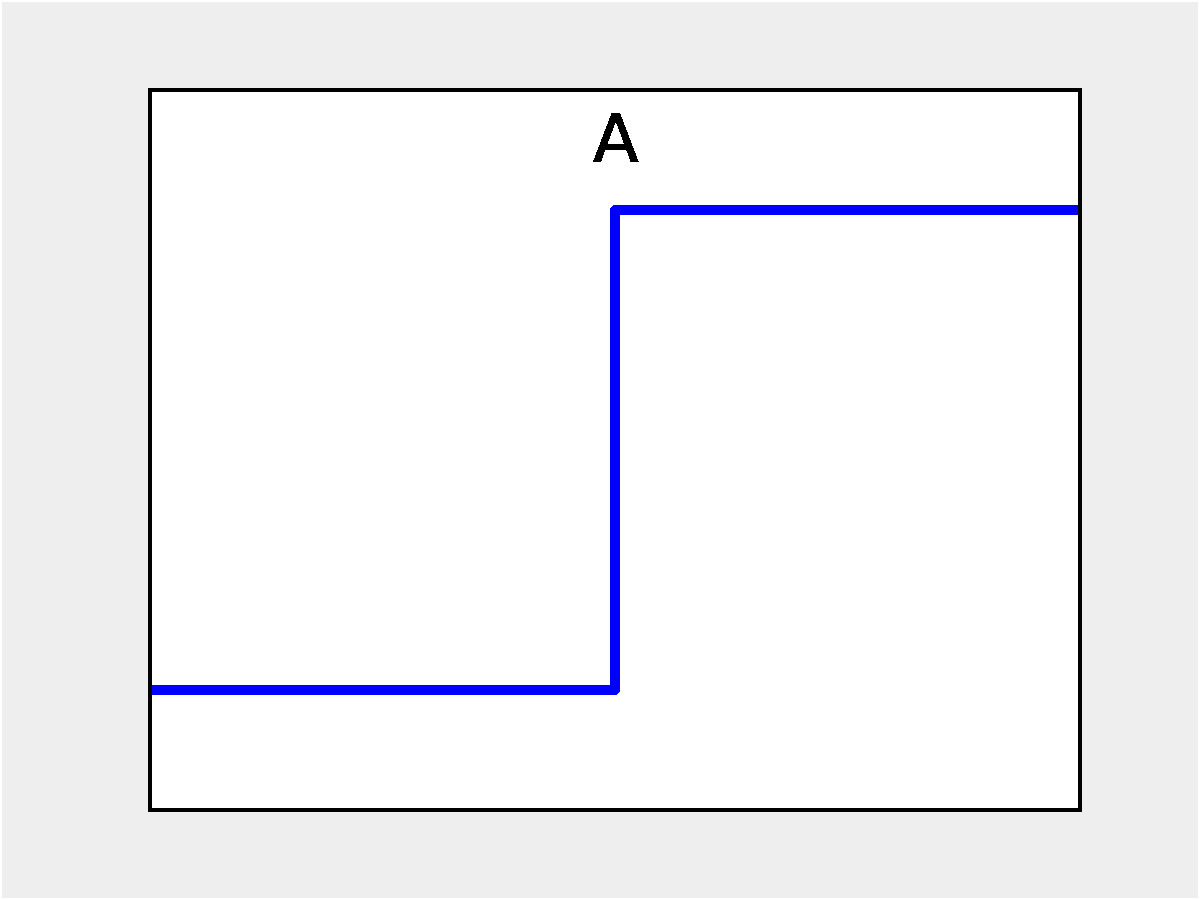
\includegraphics[width=0.3\textwidth]{figures/ch1_4_profile-heaviside}
&
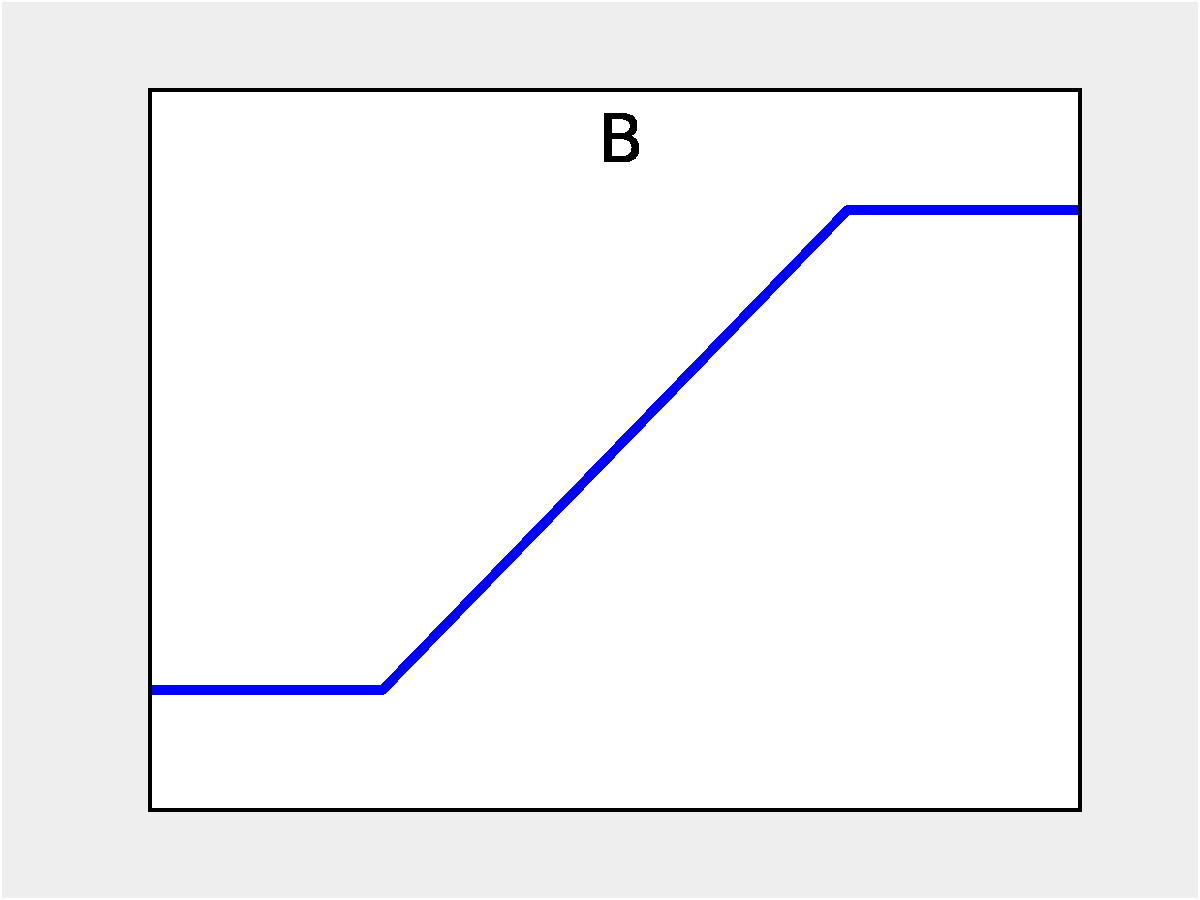
\includegraphics[width=0.3\textwidth]{figures/ch1_4_profile-linear}
&
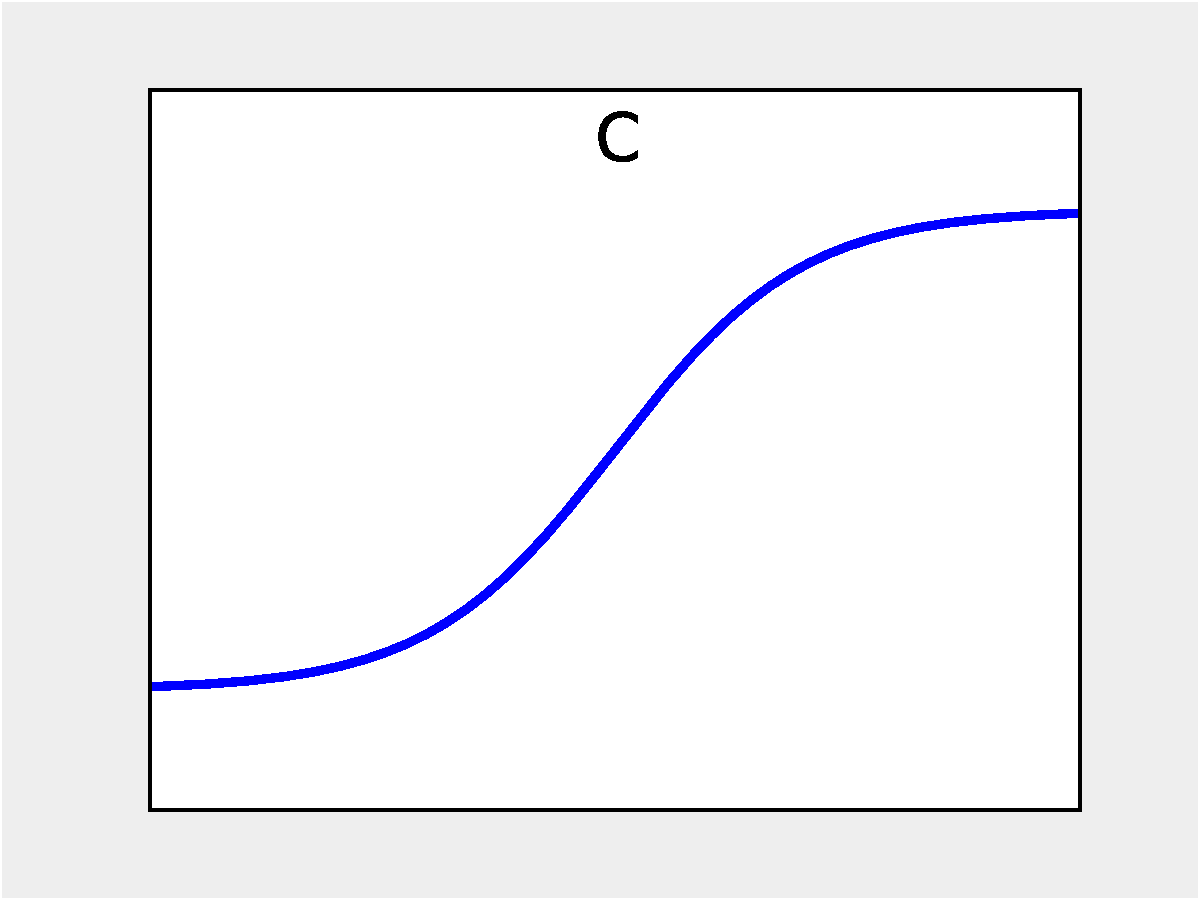
\includegraphics[width=0.3\textwidth]{figures/ch1_4_profile-sigmoid}\\
\hline
\end{tabular}
\end{center}
\caption{Exemples de fonctions de gain fréquemment utilisées pour les modèles fréquentiels. La fréquence moyenne de tir $\nu$ est représentée en fonction de la valeur de l'entrée $I$ qui peut être interprétée comme un potentiel d'action provenant d'un autre neurone. A: une fonction de Heaviside. B: une fonction linéaire par morceaux. C: une fonction sigmoïde }
\label{gain}
\end{figure}

Prenons maintenant le schéma d'interaction entre un neurone post-synaptique $i$ et plusieurs neurones pré-synaptiques $j$ tel qu'il est décrit par Ermentrout \cite{Ermentrout:1980}. $V_i(t)$ est le potentiel de membrane du neurone $i$ à l'instant t qui sera transformé en activation $\nu_i(t)=f(V_i(t))$ qui sera transmise vers d'autres neurones via l'axone.\\

Un neurone est caractérisé donc d'une part par sa fonction de gain. D'autre part, l'évolution de son état dans le temps peut être décrite par l'une des équations suivantes qui reposent sur deux approximations différentes d'une même équation globale plus complexe : 

\begin{center}
\begin{equation} 
\tau_i \frac{dV_i}{dt}+V_i= \sum_{j} {w_{ij} f_j(V_j)} 
 \end{equation}
\label{vol}
\end{center}

\begin{center}
\begin{equation} 
\tau_i \frac{dU_i}{dt}+U_i= f(\sum_{j} {w_{ij} U_j} )
 \end{equation}
\label{act}
\end{center}

La première équation est une version simplifiée du modèle intégrateur-à-fuite détaillé dans la suite. On retient que dans cette version la variable principale est le potentiel de membrane et que la fonction d'activation est à l'intérieur de la somme. La deuxième équation correspond aux modèles basés plutôt sur l'activation synaptique moyenne <U> \cite{Gutkin:2003, Wilson:1972, Pinto:1996}. Pour plus de détails voir \cite{Ermentrout:1998}.\\

Enfin, l'étude de la régularité de l'activité corticale constitue un point central dans le débat sur le codage impulsionnel ou fréquentiel. La décharge corticale a souvent été considérée comme irrégulière, proche d'un processus de Poisson, donc en faveur d'un codage impulsionnel. Mais des études récentes ont montré que la décharge d'un neurone du cortex auditif en réponse à un ton pur est plutôt binaire que Poisson \cite{DeWeese:2003}. En outre, une activité régulière de certains neurones dans les aires pariétales, en particulier le cortex moteur, a été rapportée \cite{Lee:1998, Maimon:2009}, donc en faveur d'un codage fréquentiel.\\

En résumé, l'information neuronale peut être codée de diverses manières \cite{Perkel:1968}. Les stratégies de codage fréquentiel et impulsionnel sont toujours sujettes à controverses. Les deux paradigmes semblent co-exister et selon la fonction (et la structure) étudiée, la pertinence de l'un ou l'autre l'emporte. Il en résulte donc plusieurs modèles de neurones artificiels. Nous présenterons dans la suite quelques familles de ces modèles.

\subsection{Le neurone artificiel}

\textit{Le neurone formel} est historiquement le premier modèle inspiré du neurone biologique. Le neurone formel est une fonction mathématique bornée qui prend plusieurs entrées (valeurs des variables) et donne une sortie (valeur de la fonction) qui correspondent respectivement aux dendrites du neurone biologique et son axone.\\

Le premier modèle de neurone formel a été proposé par un neurologue français appelé Louis Lapique en 1907. Des modèles plus réalistes, qui décrivent finement le fonctionnement électrique des neurones, ont été ensuite développés. Il s'agit des modèles de neurones \textit{implusionnels}. Ces modèles permettent de reproduire des mesures électrophysiologiques avec beaucoup de précision permettant donc de mettre en oeuvre un codage à spikes. D'autres modèles, comme le neurone \textit{intégrateur-à-fuite}, se basent plutôt sur le codage fréquentiel. 

\subsubsection{Neurone impulsionnel}

Les modèles impulsionnels se focalisent sur les phénomènes électriques en considérant les neurones comme des systèmes dynamiques dont la variable d'état principale est souvent \textit{le potentiel de membrane}.\\

\begin{figure}[htbp]
\begin{center}
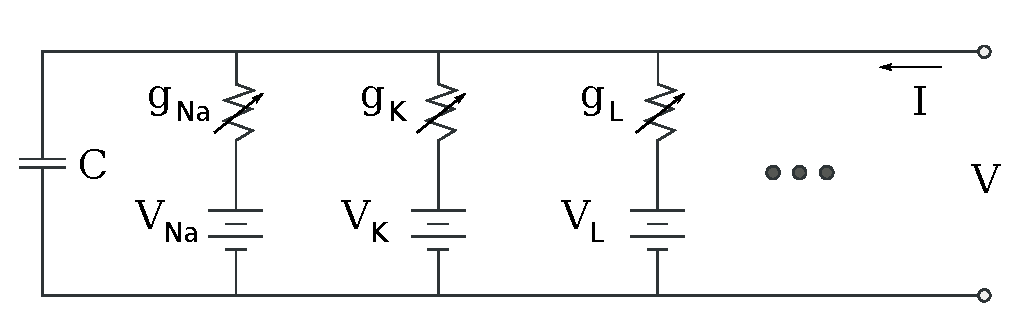
\includegraphics[width=0.5\textwidth]{figures/ch1_5_Hodgkin-huxley-circuit.pdf}
\end{center}
\caption{Schéma électrique du modèle Hodgkin-Huxley. Le courant ionique à travers la membrane peut être divisé en trois composants: courant de sodium ($I_K$), courant de potassium ($I_{Na}$) et une petite fuite de courant ($I_L$) causée par d'autres ions. Chaque composant peut être exprimé en termes de potentiel de repos de la cellule ($V$), des potentiels d'équilibre respectifs pour chaque composant ($V_K$, $V_{Na}$ et $V_L$), des constantes reflétant la conductance de chaque composant ($g_K$, $g_{Na}$ et $g_{L}$) et des variables supplémentaires ($n$, $m$ et $h$).}
\label{Hodgkin}
\end{figure}

Le modèle impulsionnel central est celui de A. Hodgkin et A. Huxley \cite{Hodgkin:1952} qui leur a valu le prix Nobel en 1963. Il décrit quantitativement comment les \textit{potentiels d'action}~(fig \ref{potentiel}) sont générés et propagés dans l'axone à travers un modèle mathématique basé sur un système d'équations différentielles couplées. Ce modèle fait intervenir des variables représentant les conductances des canaux ioniques. La membrane peut donc être représentée comme un circuit éléctrique~(voir fig.\ref{Hodgkin}).\\



\subsubsection {Neurone intégrateur-à-fuite}

Le modèle de neurone \textit{intégrateur-à-fuite} est l'un des modèles les plus populaires qui permet d'utiliser un codage fréquentiel (voir \cite{Blynel:2002} pour un aperçu sur le comportement des neurones intégrateur-à-fuite). Nous détaillerons ce modèle qui nous servira de modèle de neurone dans le chapitre 4. Il est basé sur l'hypothèse que les unités de base de calcul dans les systèmes nerveux sont les neurones individuels. L'état d'un neurone $i$ est décrit à l'instant $t$ par le potentiel de membrane $u_i$, régi par l'équation différentielle suivante :

\begin{center}
\begin{equation} 
\tau\frac{du_i(t)}{dt}= -u_i(t)+\sum_j {f(u_j(t))w_{ij}} + \sum_k {s_{ik}} +\theta
 \end{equation}
\end{center}

o\`u $\tau$ est la constante de temps. Le neurone compte une somme linéaire des entrées qu'il reçoit. La première somme s'étend sur tous les neurones $j$ qui renvoient des signaux au neurone $i$, la seconde somme s'étend sur l'ensemble des entrées externes $s_{ik}$. $w_{ij}$ décrit la force de la connexion synaptique entre les neurones $i$ et $j$. $f$ est la fonction d'activation. En l'absence d'entrées, le potentiel de membrane se relaxe vers le niveau de repos $\theta$.\\

Le terme \textit{intégrateur} décrit la capacité des neurones à intégrer l'activation entrant au fil du temps. Le terme \textit{fuite} signifie qu'une certaine quantité d'activation du neurone est perdue sur le neurone à chaque pas de temps, de sorte que son niveau d'activité décroît progressivement vers le niveau de repos en l'absence d'apport des entrées. La vitesse d'intégration des activations d'entrée et de décroissance de l'activation interne est commandée par la constante de temps $\tau$. Ainsi l'activation des neurones change de manière continue (lisse) sur plusieurs pas de temps au lieu de varier brusquement permettant ainsi de contrôler des actions plus naturelles.\\

En plus de ces modèles qui permettent de garder certaines propriétés du neurone biologique, une autre approche qui s'inspire du fonctionnement du cerveau sans chercher à le reproduire finement a été explorée. Dans ce type d'approche, la dynamique est complètement laissé de côté, seul le résultat du traitement de l'information importe. \cite{McCulloch:1943} ont proposé un modèle de neurone formel qui réalise une fonction d'intégration simple d'informations reçues des autres neurones formels. Les entrées sont pondérées par des coefficients (\textit{poids}) approchant les caractéristiques des synapses (fig\ref{Albin}). Le modèle réalise une somme pondérée des entrées suivie d'une non-linéarité (fonction de Heaviside). L'état de sortie du modèle est soit $0$, soit $1$ (activé ou non-activé). Les auteurs distinguent les entrées excitatrices des entrées inhibitrices. Une variante du modèle consiste à utiliser des poids négatifs pour les entrées inhibitrices et des poids positifs pour les entrées excitatrices. Ensuite si la somme dépasse une valeur seuil prédéfinie, la sortie sera $1$, sinon $0$.\\

\begin{figure}[htbp]
\begin{center}
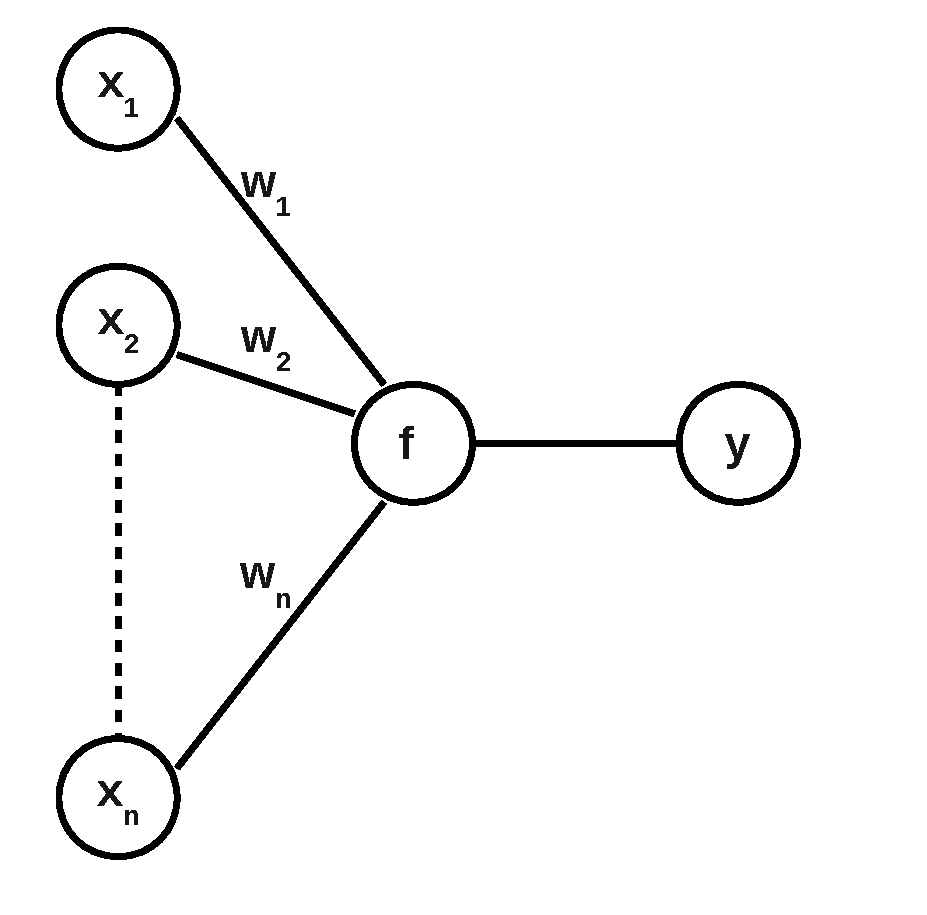
\includegraphics[height=0.3\textwidth]{figures/ch1_6_formel}
\end{center}
\caption{Le neurone formel réalise une fonction non linéaire bornée qui prend plusieurs entrées $x_i$ (entrées pré-synaptiques) pondérées par des poids de connexion $w_i$ et retourne une sortie (sortie post-synaptique) $ y = f (x_1, x_2, ..., x_n; w_1, w_2, ..., w_n)$. }
\label{formel}
\end{figure}

Enfin, le neurone comme unité isolée reste une fonction simple qui n'a pas d'énormes capacités de calcul. C'est l'association de tels éléments simples sous la forme de réseaux qui permet de réaliser des fonctions utiles permettant de résoudre des problèmes complexes. On passe donc à un codage permettant de faire des calculs distribués, o\`u chaque unité détient une partie de l'information.\\

En particulier, McCulloch et Pitts ont montré comment des systèmes neuronaux pourraient mettre en œuvre une logique du premier ordre. Influencés par les travaux de Nicolas Rashevsky dans les années 1930 qui suggère que le cerveau pourrait être vu comme une organisation de 0 et de 1 (la première édition de son livre \textit{Mathematecal biophysics} en 1938), ils ont introduit des réseaux de neurones discrets dans le temps et avec des variables booléennes comme un modèle du fonctionnement du cerveau. Cela nous amène à la théorie connexionniste résultant des deux constatations suivantes: D'une part, la mise en commun d'unités simples permet d'acquérir de vastes capacités de traitement de l'information \cite{Rashevsky:1960}, d'autre part, \cite{Hebb:1949} a introduit une règle d'apprentissage décrivant comment les interactions entre plusieurs neurones permet de modifier le comportement de l'ensemble.


\section{Approche connexionniste: Les réseaux de neurones}

La théorie du \textit{connexionnisme} issue des travaux de \cite{Hebb:1949, Hayek:1952} est une approche qui modélise les fonctions cognitives complexes comme des processus émergents d'un ensemble d'unités simples interconnectées utilisant des calculs locaux simples. Cet ensemble d'unités forme ce qu'on appelle un \textit{réseau de neurones}. La forme des connexions et les caractéristiques des unités peuvent varier selon les modèles. Par abus de langage on confond souvent les termes neurone (biologie), unité (unité de calcul), cellule (automate cellulaire) et neurone artificiel (connexionisme).\\

Le \textit{perceptron} est l'un des premiers réseaux de neurones artificiels, il résulte des travaux de Rosenblatt \cite{Rosenblatt:1958}. C'est un modèle inspiré du système visuel. Il est constitué de seulement deux couches de neurones, une couche d'entrée (dite \textit{perceptive}) qui correspond aux neurones sensoriels qui reçoivent les stimuli du monde externe et une couche de sortie (dite \textit{décisionnelle}) qui correspond aux neurones moteurs qui restituent les résultats au monde externe. Les neurones de la couche d'entrée projettent sur les neurones de la couche de sortie selon des jonctions (des connexions). On associe un poids synaptique à chaque jonction, de sorte que les entrées sont multipliés par ce poids, puis additionnées par les neurones de sortie, ce qui est équivalent à multiplier le vecteur d'entrée par une matrice de transformation.\\

Dans ce type de réseaux les connexions se font dans un seul sens (\textit{feedforward}) par opposition aux réseaux dit \textit{récurrents} \cite{McCulloch:1943} dans lesquels les sorties de certaines unités sont retournées vers des unités de la couche d'entrée. En plus, il est supposé implicitement qu'il n'y a pas d'organisation spatiale des connexions. Cependant, il existe dans le cortex et dans d'autres régions cérébrales des répartitions spatiales claires des connexions entre les différentes unités neuronales. Nous examinerons dans la suite des modèles de réseaux de neurones dynamiques qui prennent en compte ces constatations.\\

En effet, le nombre de neurones et de synapses dans une petite partie du cortex étant immense, l'hypothèse de considérer une couche de neurones comme un continuum dans l'espace a été adoptée par plusieurs chercheurs dans le cadre de la théorie des champs neuronaux continus (CNFT, \textit{continuum neural field theory}) \cite{Wilson:1973, Amari:1977}. Cette théorie s'inspire de la théorie \textit{des champs continus} en physique défendue par Albert Einstein. L'évolution de l'état interne du champ neuronal est décrite par une équation différentielle dépendant de l'espace et du temps. Le profil des connexions dépend lui aussi du positionnement dans l'espace.\\

Considérons la version généralisée d'un champ neuronal dynamique (DNF, \textit{dynamic neural field}) avec des délais de transmission, qui décrit l'évolution spatio-temporelle du potentiel de membrane dans une population de neurones. Nous allons considérer un seul réseau (\textit{champ}) $M$ composé de plusieurs unités avec des connexions spatiales entre elles. Chaque unité, au niveau mésoscopique biologique, peut correspondre à une colonne corticale \cite{Chemla:2007}. Le réseau représente donc une carte corticale (voir par exemple \cite{Vieville:2007} pour une discussion sur le concept), et peut être modélisé par un DNF continu dans l'espace \cite{Wilson:1973, Taylor:1999, Amari:1977}. L'évolution du potentiel de membrane $ V $ d'une unité dans un tel réseau est décrite par l'équation différentielle suivante:\\
%%
\begin{align}
  \label{eq: DNF-continuous}
  & \frac{\partial V(\mathbf{x},t)}{\partial t} =
  -\frac{1}{\tau(\mathbf{x})} \, V(\mathbf{x},t) + h(\mathbf{x}, t) + s(\mathbf{x}, t) 
  &+ \int_{\cal M} d \mathbf{y} \, \int_0^{+\infty} \, \hspace{-1em} d \eta \; W(\mathbf{x}, \mathbf{y}, \eta) \, \sigma_{\mathbf{y}}\left(V(\mathbf{y}, t - \eta)\right) 
\end{align}
%%

où $\mathbf {x}$ désigne une position dans le champ continu $M$, $t$ est le temps, $V(\mathbf{x},t)$ désigne le potentiel de membrane au point $\mathbf {x}$ à l'instant $t$, $ {\tau} $ est la constante temporelle caractéristique des synapses, $\eta$ est le délai de transmission, $ W $ est la fonction de connexions synaptiques, $ s(\mathbf {x},t) $ est l'entrée reçue à la position $ \mathbf {x} $ et $ h $ est le seuil moyen du neurone. Dans ce cadre, $ \sigma_ {\mathbf{y}} ()$ est une fonction sigmoïde qui représente la fonction d'activation du neurone à la position $y$. \\

Certains modèles de DNF supposent que la vitesse de transmission des signaux dans le réseau n'est pas bornée, donc négligent les délais de transmission (i.e., $W({\bf x}, {\bf y}, \eta) = w({\bf x}, {\bf y}) \, \delta(\eta - 0)$, avec seulement des transmissions \textit{instantanées}). D'autres considèrent une transmission constante, avec un retard (e.g., $W({\bf x}, {\bf y}, \eta) = W({\bf x}, {\bf y}) \, \delta(\eta - \frac{|{\bf x} - {\bf y}|}{v})$ pour une vitesse de propagation $v$). La formulation précédente englobe ces différents cas, en tenant compte de la nature spatio-temporelle de la connexion. \\

Enfin, l'un des principaux intérêts des réseaux connexionnistes est leur capacité d'\textit{apprentissage}. Biologiquement, il s'agit de modifier la transmission synaptique, ce qui nous ramène à la notion de \textit{plasticité synaptique}.  Il s'agit d'une sous-partie d'une propriété plus large du réseau neuronal et du cerveau en général: la plasticité neuronale (ou cérébrale). Le cerveau est qualifié donc de ``plastique'' (en perpétuelle reconfiguration), il se modifie et s'adapte par l'expérience. Nous examinerons cette notion dans la section suivante.\\


\section {Calcul adaptatif : Plasticité et apprentissage}
 

La plasticité synaptique repose sur le fait que l'efficacité d'une synapse peut varier au cours du temps. Elle englobe tous les mécanismes intervenant dans la modification de la transmission synaptique au cours du temps. En effet, la connexion entre deux neurones n'est pas figée mais dépend de l'activité précédente des neurones et de l'utilité de cette connexion dans la génération du résultat final. \\

La première règle proposée pour la plasticité, dans le cadre de l'apprentissage, est celle de Hebb \cite{Hebb:1949, Gerstner:2002} qui postule qu'une synapse devient plus efficace quand elle participe à l'activation du neurone post-synaptique. Ce postulat implique que l'augmentation de l'efficacité synaptique nécessite une corrélation temporelle entre l'activation des deux neurones (décharger de manière rapprochée) qui peut traduire un lien de causalité. La règle d'apprentissage de Hebb se formule de la manière suivante \textit{``quand une cellule A excite de manière répétée une cellule B, l'efficacité de A à exciter B est améliorée par des changements métaboliques''}. Considérons une synapse avec une efficacité $w_{ij}$ permettant de transmettre des signaux d'un neurone pré-synaptique $i$ vers un neurone post-synaptique $j$. On se contente ici de la formulation en termes de fréquence moyenne de décharge. Dans la suite, l'activité du neurone pré-synaptique est notée $\nu_i$ et celle du neurone post-synaptique est notée $\nu_j$. La variation de l'efficacité synaptique, selon la règle de Hebb, est donnée par l'équation générale suivante:\\

\begin{align}
\frac{\delta w_{ij}}{\delta t}=G(w_{ij};\nu_i,\nu_j)
\end{align}

Cette formulation souligne le caractère local de la règle, mais un autre aspect important du postulat de Hebb est l'effet cooperatif. Ils faut que les neurones pré- et post-synaptiques s'activent simultanément pour que le poids synaptique change. D'o\`u l'exemple particulier de la fonction $G$ dans l'équation suivante:

\begin{align}
\frac{\delta w_{ij}}{\delta t}=\alpha \nu_i \nu_j
\end{align}

 où la variable $\alpha$ est appelée le coefficient d'apprentissage.\\

Dans la version initiale, seul le renforcement est envisagé ($\alpha >0$) et en absence de mécanisme complémentaire, les synapses seraient saturées à leur poids maximal. C'est ainsi qu'un postulat complémentaire a été proposé par \cite{Stent:1973}:\textit{"Quand un neurone pré-synaptique A échoue de manière répétée et persistante à exciter un neurone B post-synaptique tandis que cette cellule décharge sous l'influence d'autres neurones pré-synaptiques, un changement métabolique se produit dans la voie entre les deux cellules de manière à ce que l'efficacité de A est diminuée"}. On parle donc de \textit{dépression synaptique}.\\

Plus généralement, il s'agit d'une règle d'apprentissage \textit{non-supervisé} (apprendre sans professeur) qui sera décrite brièvement dans la suite ainsi que les deux autres types d'apprentissage : \textit{supervisé} (apprendre à trouver la bonne réponse à une demande spécifique) et \textit{par renforcement} (apprendre par interaction avec l'environnement via la récompense).\\

\subsection{Apprentissage supervisé}

L'apprentissage supervisé consiste à apprendre une tâche en se basant sur l'erreur entre la réponse fournie par le modèle et la réponse attendue connue par l'expérimentateur (le professeur). Ce dernier doit fournir au système un échantillon d'entrées possibles ainsi que les réponses désirées correspondant à ces entrées. Pour chaque entrée, le réseau fournit une réponse qui sera comparée à la réponse désirée, ensuite les poids sont ajustés de manière à ce que la sortie soit le plus proche possible de la réponse désirée si cette entrée est présentée prochainement. %Ce mode d'apprentissage est le moins plausible biologiquement.

\subsection{Apprentissage non-supervisé}\label{AS}



L'apprentissage non supervisé est une méthode d'apprentissage automatique qualifiée aussi d'associative. Dans l'échantillon d'apprentissage les sorties désirées ne sont pas connues. Les seuils d'activations et les poids sont modifiés en fonction du rapport de causalité entre les activités des unités comme dans le mécanisme proposée par Hebb \cite{Hebb:1949}. Il s'agit donc d'un apprentissage de corrélations.\\

Quand l'apprentissage (supervisé ou non) est terminé, le réseau est testé sur de nouvelles entrées. Si les performances du réseau sont jugées bonnes sur ces nouvelles entrées, on dit que le réseau a pu généraliser à partir des exemples qui ont servi à l'apprentissage.\\

\subsection{Apprentissage par renforcement}

L'apprentissage par renforcement (RL, \textit{Reinforcement learning}) est l'apprentissage par interaction avec un environnement. Le modèle (l'agent) est enseigné de manière implicite en se basant sur les expériences passées (l'exploitation) et sur les nouveaux essais (l'exploration). Il apprend donc les conséquences de ses actions qu'il reçoit sous forme de récompense numérique\footnote{L'utilisation du terme de la récompense est utilisé ici de façon neutre et n'implique pas de plaisir ni aucune autre interprétation psychologique.} codant sa réussite \cite{Sutton:1998, Barto:1995}. Le but est de maximiser la récompense cumulée au fil de temps. \\

Ces trois modes d'apprentissage sont plus ou moins biologiquement plausible et semblent co-exister dans le cerveau. Doya propose que le cervelet peut assurer un apprentissage supervisé, contrairement aux noyaux gris centraux (appelés encore les ganglions de la base), qui peuvent effectuer un apprentissage par renforcement, et le cortex cérébral un apprentissage non supervisé \cite{Doya:2000}. \\

Mais la complexité des systèmes étudiés rend l'étude théorique de leur évolution ainsi que la mise en oeuvre de ces schémas d'apprentissage difficiles. En effet, la résolution analytique des équations différentielles qui les régissent est souvent compliquée voire impossible. Donc la solution est de simuler numériquement l'évolution en passant obligatoirement par une approximation discrète du système étudié. À ce stade, il est important de noter qu'un tel modèle possède trois niveaux distincts de continuité, à savoir: l'espace, le temps et la valeur de la variable de base. C'est pourquoi nous nous sommes intéressés aux problèmes de discrétisation dans le cadre des DNF comme détaillé dans la section suivante.\\

%%%%%%%%%%%%%%%%%%%%%%%%%%%%%%%%%%%%%%%%%%%%%%%%%%%%%%%%%%%%%%%%%%%%%%%%%%%%%%%%%%%%%%%%%%%%%%%%%%%%%%%%%%%%%%%%%%%%%%%%%%%%%%%%%%%%%%%%%%
\section{Intégration numérique: Champs neuronaux discrets }

Ici, nous considérons le niveau de discrétisation spatial comme un a priori. Nous examinerons brièvement le problème de discrétisation de la variable principale puis nous nous concentrerons sur la discrétisation temporelle. Nous pouvons maintenant réécrire l'équation de l'évolution de l'état des unités discrètes, indexées par un ensemble fini $M$ (ce qui correspond à l'échantillonnage spatial du champ continu $M$ dans l'équation précédante):\\

\begin{align}
\label{eq: DNF-discret}
  \frac{\Delta V_i(t) }{\Delta t}  = &- L_i \, V_i(t)  + I_i(t)+\sum_{\substack{j \in M\\k \in \{k_{\min}, k_{\max}\}}} \hspace{-1em} W_{ijk} \, \sigma_j\left(V_j(t - k\, \Delta T)\right)
\end{align}

Ici $V_i(t) \equiv V(\mathbf{x}_i, t)$ désigne l'état mésoscopique à l'endroit échantillonné $\mathbf{x}_i$  (à savoir la moyenne spatiale du potentiel de membrane, pour la sous-population de neurones dans cette position à l'instant t). $L_i \equiv \frac{1}{\tau(\mathbf{x}_i)}$ est le terme de fuite (lié à la constante de temps caractéristique de la dynamique des synapses ), tandis que $\sigma_j()$ est la même fonction définie dans~(\ref{eq: DNF-continuous}), et $W$ représente le poids de connexions. Les poids sont indexés par les index spatiaux et par l'indice du retard $k$ compris entre $k_{min}$ et $k_{max}$. Enfin $I_i(t) \equiv h(\mathbf{x}_i, t) + s(\mathbf{x}_i, t)$ englobe à la fois $s(\mathbf{x}_i, t)$ et le seuil moyen d'activation $h(\mathbf{x}_i, t)$.\\

En outre, un point important est la distinction entre l'échantillonnage de temps de simulation $ \Delta t $ et l'échantillonnage de temps de modélisation $ \Delta T $. Le choix de l'échantillonnage de l'intégrale $ \int_0 ^ {+ \infty} \, d \eta $ (équation \ref{eq: DNF-continuous}) par une somme  $ \sum_ {k = k_ {\min}} ^ {k_ {\max}} $ à $ t = k \Delta T $  est un choix de modélisation, alors que le calcul de la fraction $ \ {\partial V (\mathbf {x}, t)} {\partial t} $ (équation \ref{eq: DNF-continuous}) à un taux de $ \Delta t $ est une question de simulation.\\

L'équation précédente~(\ref{eq: DNF-continuous}) correspond au champ de neurones dynamique (voir, par exemple, \cite{Grimbert:2008} pour une revue récente) et l'équation~\ref{eq: DNF-discret} correspond à une population discrète de neurones équivalente et nous allons seulement considérer ce dernier système dans ce qui suit. Puisque la résolution analytique des équations différentielles telles que l'équation~\ref{eq: DNF-discret} n'est pas toujours possible, l'évolution du système peut être approchée en utilisant l'intégration numérique. \\


\subsection{Discrétisation des valeurs}

Même si une variable numérique prend un nombre fini de valeurs, il est important de souligner que cette contrainte ne sera pas prise en compte dans notre étude. Examinons donc brièvement ce niveau de discrétisation.\\

Un système dynamique discret (DDS, \textit{discrete dynamic system}) est un ensemble fini d'éléments, ayant un nombre fini d'états, évoluant dans un temps discret grâce à des interactions mutuelles. Dans \cite{Robert:1994}, la dynamique temporelle de ces systèmes est analysée. Prenons comme exemple de DDS  un automate cellulaire avec $N $ cellules booléennes (un nombre fini d'états $\{0,1\}$), qui peut correspondre dans un réseau neuronal à un état actif du neurone (spiking) ou à un état ​​silencieux (repos). Plus précisément, à partir d'un état ​​initial à $ t = 0 $, à chaque pas de temps, chaque unité met à jour son état ​​d'activation en se basant sur les états du sous-ensemble d'unités qui lui sont connectées.\\

Un tel système n'est pas suffisant pour modéliser les DNF, qui représentent des quantités physiques dont l'évolution est décrite par des équations différentielles avec des variables continues. Mais il reste utile dans la mesure o\`u il permet de donner des estimations qualitatives des comportements simulés par les DNF (voir \ref{convergence}).\\


%
\subsection{Discrétisation du temps}

Considérons d'abord le cas très simple d'une approximation linéaire constante du système~(\ref{eq: DNF-discret}) avec la condition initiale $ V_j (0) $, dans le cas particulier où le terme de fuite $ L_j $, la fonction de poids $W_{jk0} $ et l'entrée courante $I_j$  sont constants, les retards de transmission sont négligés, tandis que  $\sigma_j\left(u\right) = u$ (voir \cite{Alexandre:2009} pour une discussion sur les profils de sigmoïde habituellement utilisés). Ce qui donne en forme vectorielle l'équation suivante:\\
\begin{align}
\frac{\Delta V(t)}{\Delta t} = -{ W} \, { V}(t) + { I},
\end{align}
avec
%%
\begin{align}
\label{eq: def-W}
{ W} \equiv \left(\begin{array}{ccc} L_1 & -W_{120} & \cdots \\ -W_{210} & L_2 & \cdots \\  \cdots & \cdots & \cdots \\ \end{array} \right), \;
{ I} \equiv \left(\begin{array}{c} I_1 \\ I_2 \\ \cdots \\ \end{array} \right),
\end{align}
%%
et après un échantillonnage régulier selon l'approximation d'Euler\footnote{Cette méthode, sur une équation d'ordre 1 de type $y' = f(x,y)$, consiste à prendre localement pour approximation de $y(t_0+h$), en $t_0+h$, la valeur $y(t_0) + h*y'(t_0)$. Autrement dit, localement on approxime la courbe par sa tangente. Il s'agit d'un cas particulier de la méthode Runge-Kutta qui est définie par: $
y_{i+1}=y_{i}+h\varphi(x_{i},y_{i},h), y_{0}=y(x_{0}) $. Pour la méthode d'Euler on a  $\varphi=f $ . L'objectif de Runge-Kutta est d'obtenir une meilleure précision grâce au degré de liberté supplémentaire que constitue le choix de la fonction $\varphi $. Nous nous restreindrons à l'approximation du $1^{er}$ ordre, d'Euler.} \cite{Press:1988} l'équation s'écrit:\\

\begin{center}$ V[i+1] = { V}[i] + \Delta t \, \frac{\Delta V(t)}{\Delta t},$ à l'instant $t = i \Delta t,$ \\\end{center}

Ici, nous ne considérons que le cas où le système converge vers une solution stable, c'est à dire le cas du système \textit{contractant} où les parties réelles des valeurs propres de ${W}$ sont strictement positives impliquant que la matrice ${W}$ est diagonalisable. Dans ce cas, si cette approximation d'Euler converge, cela sera forcément vers la solution continue (\cite{Press:1988}). Autrement dit, cela signifie que le terme de fuite est assez fort (par rapport aux poids) pour induire la convergence du système, (voir \cite {Alexandre:2009} pour une étude détaillée dans le cas de champs neuronaux discrets). Plus précisément, sur une direction propre (c'est à dire dans la direction d'un vecteur propre de la matrice), l'équation linéaire est découplée des autres et le terme de fuite (soit un réel ou une valeur complexe) correspond à l'opposé de la valeur propre. \\
 
\begin{figure}[htbp]
\begin{center}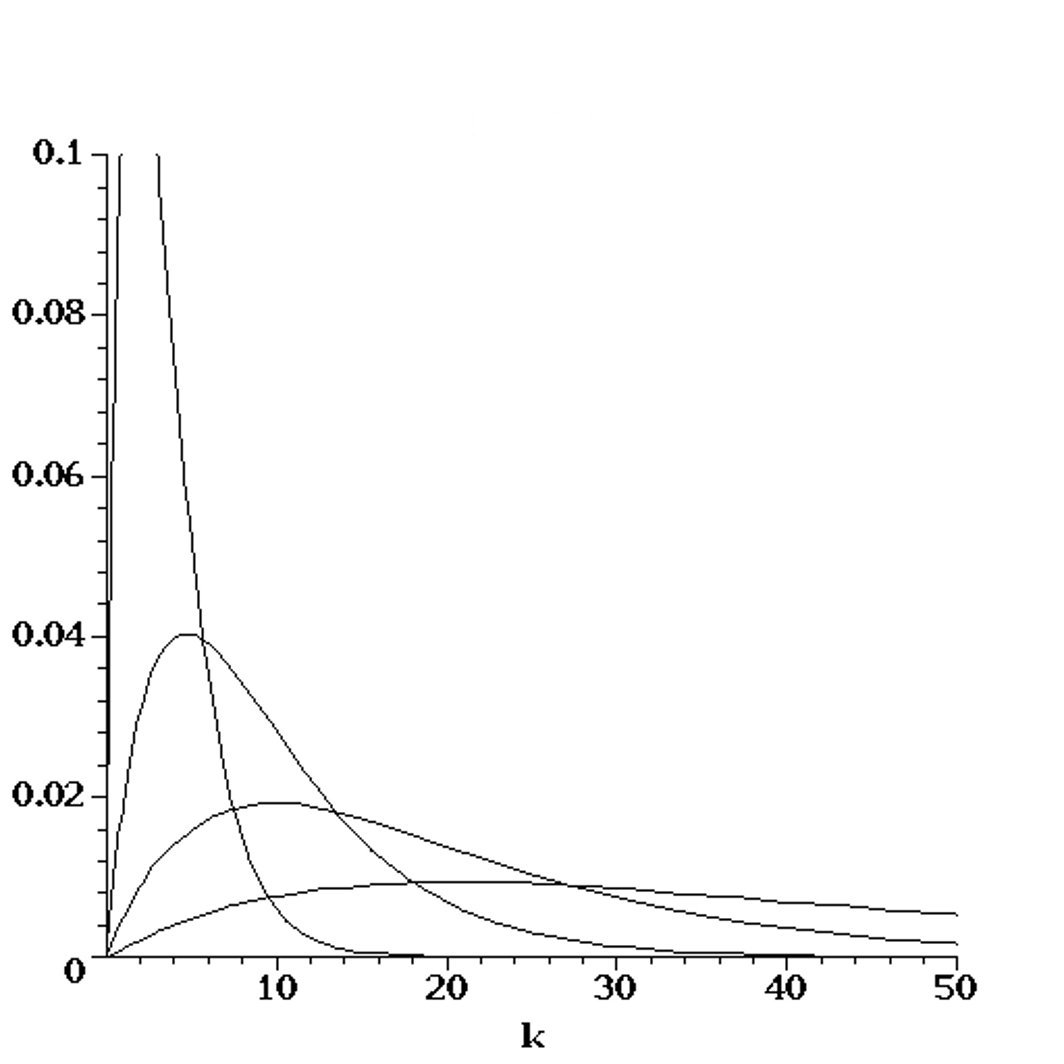
\includegraphics[width=0.35\textwidth]{figures/ch1_7_biais.jpeg}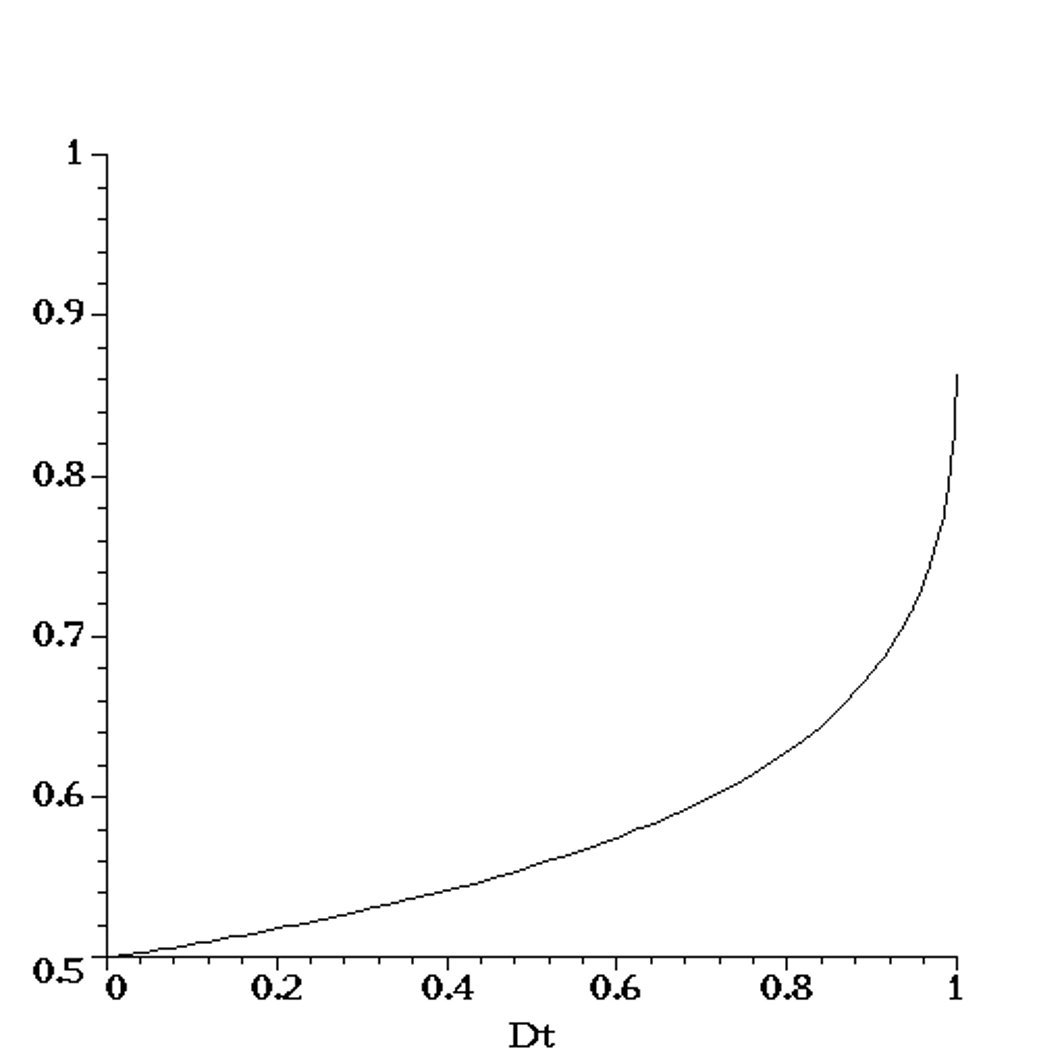
\includegraphics[width=0.35\textwidth]{figures/ch1_7_integralbiais.jpeg}\end{center}
\caption{{\em \`A gauche}: Le profil temporel normalisé du biais de calcul entre le schéma continu et son approximation discrète pour $\Delta t / \tau_j = [0.05, 0.1, 0.2, 0.5]$ en partant de la courbe la plus plate à la plus pointue .
{\em \`A droite}: L'intégral du biais le long de la trajectoire en fonction de $Dt=\Delta t / \tau_j$, en explicitant que l'écart systématique cumulatif n'est jamais négligeable, même pour des valeurs très faibles du terme de fuite, alors qu'il diverge pour les valeurs importantes. Voir le texte pour plus de détails.}
\label{fig: euler-error} 
\end{figure} 


Dans un tel cas, le schéma continu et son approximation discrète convergent vers le même point fixe en partant de la même valeur initiale, mais pas selon la même trajectoire. Plus précisément, le biais dans une direction propre de la matrice $ {W} $ est proportionnel à $ V_j (0) - I_j \, \tau_j$, où $ 1 / \tau_j $ est la valeur propre (qui correspond au terme de fuite) dans cette direction, et suit le profil d'une exponentielle double (fonction de $\Delta t / \tau_j$), comme illustré dans la figure~\ref{fig: euler-error}. Autrement dit, plus $\Delta t / \tau_j  \in [0, 1 [$ (les bornes correspondant à l'intervalle de convergence) est élevé, plus l'écart entre les deux schémas (continu et discontinu) est important, mais moins la durée du biais (la durée pendant laquelle le biais est non nul) est importante.\\

Il s'agit d'un résultat contre-intuitif et très important de noter que les grandes valeurs du terme de fuite (constantes de temps faibles) accélèrent la convergence. Mais il reste l'inconvénient de générer des erreurs importantes au cours des premières itérations. Même dans un tel cas très simple, au début de la trajectoire, l'approximation discrète du système dynamique continu peut très bien ne pas converger vers l'attracteur attendu du système continu (voir la courbe discontinue correspondant à $\Delta t / \tau_j = 0.05$ fig.~\ref{fig: euler-error}), mais vers un autre comme on l'observe dans \cite {Rougier:2009}.\\

Dans le cas plus général o\`u le terme de fuite, les poids ou les entrées varient avec le temps, les résultats précédents se généralisent compte tenu du fait que le terme de fuite est borné. Dans le cas non-linéaire, les résultats précédents se généralisent aussi en délimitant la fonction non-linéaire $\sigma_ {j}$ par la fonction linéaire correspondante de pente maximale (voir, \cite {Cessac:2007}) pour un examen de ces outils). \\%Plus précisément, si le système est hyperbolique, la même condition s'applique sur la Jacobienne du système à tout moment et pour toute valeur.\\

En conséquence, nous apprenons de cette courte analyse que, généralement, même si le schéma continu et le schéma discontinu peuvent converger vers le même point fixe, ils ne convergent pas selon la même trajectoire. Dans tous les cas, l'écart systématique cumulatif n'est jamais négligeable.\\
%%%%%%%%%%%%%%%%%%%%%%%%%%%%%%%%%%%%%%%%%%%%%%%%%%%%%%%%
%%%%%%%%%%%%%%%%%%%%%%%%%%%%%%%%%%%%%%%%%%%%%%%%%%%%%%%%%%%%%%%%%%%%%%%%%%%%%%%%%%%%%%%%%%%%%%%%%%%%%%%%%%%%%%%%%%%%%%%%%%%%%%%%%%%%%%%%%%%%%%%%%%%%%%

Il en résulte donc que lors de la simulation d'un système à temps continu régie par une équation différentielle, le choix du schéma de discrétisation détermine la précision des trajectoires de son évolution (la précision de la dynamique) même si l'état final est souvent conservé. Le problème est que plus on essaye d'approcher le schéma de discrétisation du schéma continu, plus la mise en oeuvre est compliquée et couteuse en termes de ressources de calcul. Donc c'est l'objectif des travaux de simulation qui impose le niveau de détail et de précision à choisir pour maximiser le rapport qualité/prix.

%%%%%%%%%%%%%%%%%%%%%%%%%%%%%%%%%%%%%%%%%%%%%%%%%%%%%%%%%%%%%%%%%%%%%%%%%%%%%%%%%%%%%%%%%%%%%%%%%%%%%%%%%%%%%%%%%%%%%%%%%%%%%%%%%%%%%%%%%%%%%%%%%%%%
\section{Calcul distribué: A-t-on vraiment besoin d'une horloge centrale?}

Quelle que soit la méthode numérique utilisée pour résoudre les équations différentielles qui décrivent l'évolution du système, il est supposé implicitement qu'il y a une horloge centrale pour synchroniser les calculs. Par exemple, pour calculer les variables du modèle à l'instant $t$, les méthodes explicites utilisent l'information disponible sur toutes les variables du modèle à l'instant $t-\Delta t$. La connaissance de quelle unité a été mise à jour à tel instant $V(i)$ doit donc être centralisée pour pouvoir donner le signal permettant de passer à la prochaine étape $V(i+1)$.\\

Quelles sont les conséquences? Au niveau informatique, cela signifie que si nous utilisons une architecture multi-processeurs, les processeurs qui terminent leur tâche en premier doivent attendre à ne rien faire, jusqu'à ce que les autres finissent. Au niveau du système dynamique, ces mises à jour régulières peuvent induire des mécanismes de synchronisation parasites. En effet, des simulations ont montré que des états synchronisés peuvent appraître rapidement dans des réseaux de neurones impulsionnels réciproquement couplés \cite{Hopfield:1995}. Au niveau de la modélisation biologique, si l'on suppose l'existence d'une horloge globale universelle, qui est une approximation raisonnable pour les petits systèmes dynamiques, il est moins évident lorsque l'on considère plusieurs cartes corticales en interaction avec des délais de transmission complexes.\\

Mais puisque la caractéristique de base des réseaux de neurones est de pouvoir assurer un calcul distribué (chaque neurone détient une partie de l'information), il est assez contre-intuitif de s'appuyer implicitement sur une telle horloge centrale. Dans ce contexte, nous tenons à étudier dans quelle mesure nous pouvons éliminer cette horloge centrale et mettre en oeuvre un calcul plutôt \textit{asynchrone} dans le cadre des DNF, ce qui a déjà été étudié dans le cas des automates cellulaires \cite{Fates:2005, Fates:2008, Garcia:2006, Barret:1999, Robert:1994} et les calculs parallèles\cite{Bertsekas:1991, Bertsekas:1997} où les différents niveaux de synchronie numérique ont été pris en compte.\\ 


\subsection{De l'\'evaluation synchrone vers l'\'evaluation asynchrone }

Le calcul synchrone se réfère à la méthode numérique standard utilisée pour résoudre un ensemble d'équations différentielles \textit{ordinaires}. Après avoir choisi une résolution temporelle $ \Delta t $, une valeur $ V_i (t + \Delta t)$ est évaluée en fonction de $ V_i (t) $ et $ \Delta V_i (t) / \Delta t $ en utilisant une des nombreuses méthodes implicites ou explicites disponibles (Euler, Runge-Kutta, etc.).\\ 

Puisque n'importe quelle valeur $ V_i (t + \Delta t) $ dépend de la valeur de $V_j$ à des moments antérieurs et peut notamment dépendre de $ V_j (t + \Delta t)$, il est important de mettre à jour $ V_i (t)$ une fois que toutes les valeurs $ V_j (t + \Delta t) $ sont connues. En d'autres termes, chaque unité calcule son état suivant sans l'afficher, puis toutes les unités changent leur état actuel ($ V_i (t) $) en ($ V_i (t + \Delta t $) simultanément. Cela nécessite donc un contrôle centralisé signalant les unités qui sont autorisées à mettre à jour ``publiquement'' leur état. Même si tous les états ne sont pas modifiés à chaque étape, comme par exemple avec la méthode de Gauss-Seidel \cite {Bertsekas:1991}, l'horloge centrale est toujours nécessaire (parce que nous devons nous assurer que chaque unité a été mise à jour exactement une fois), donc le calcul reste macroscopiquement synchrone dans ce sens. \\

Un système \textit{totalement asynchrone} implique donc de contourner une telle horloge globale et de laisser le système fonctionner sous un contrôle entièrement distribué. D'un point de vue informatique, cela signifierait que chaque processeur est une unité indépendante avec une notion locale de temps et est donc mis à jour séparément. D'un point de vue biologique, cela refléterait plusieurs aspects:\\

\begin {itemize}
\item Une asynchronie entre les éléments à mettre à jour générée par les délais de communication liés aux durées de traitement et de transmission.\\

\item Une asynchronie adaptative, c'est à dire le fait qu'une unité adapte l'évaluation de son état: plus sa valeur est stable, moins de mises à jour seront faites. Ici l'asynchronisme est utilisé comme un outil computationnel.\\

\item Des événements mésoscopiques comme le changement soudain d'activité et l'influence des événements extérieurs. Ici l'asynchronisme devient liée à certaines fonctionnalités du système.\\
\end {itemize}

A ce niveau de modélisation, où le traitement de l'information est un aspect clé du calcul neuronal, nous pouvons avoir des temps d'exécution différents et des unités qui ne sont pas sensées attendre que les autres finissent leur traitement. En outre, les délais de transmission contribuent à désynchroniser les informations échangées. Les deux phénomènes sont à prendre en compte dans un paradigme \textit{totalement asynchrone}. En d'autres termes, l'asynchronisme n'est pas seulement un problème d'implémentation, il est également un problème de modélisation.\\

\subsection{Le paradigme de calcul asynchrone}\label{paradigme}

\cite {Mitra:1987} présente un travail important sur l'informatique asynchrone qui aborde le sujet un niveau très général. Son approche originale s'inspire de l'ouvrage de \cite{Chazan:1969} qui propose et analyse des algorithmes asynchrones à utiliser dans des processeurs parallèles, entre autres pour la résolution de systèmes d'équations linéaires, non linéaires ou d'équations différentielles. Ces deux références proposent un certain nombre de résultats de convergence. En suivant les travaux de Mitra \cite{Mitra:1987}, nous proposons le paradigme de calcul asynchrone suivant: le calcul est divisé en unités locales qui envoient leur résultat vers les autres unités dès que leur calcul est achevé. A chaque unité d'indice $i$ correspond une approximation de l'équation~(\ref{eq: DNF-discret}).\\

Plus précisément, à un moment donné d'échantillonnage d'indice $k$, seul un sous-ensemble d'unités choisies arbitrairement $S(k)$ est évalué. $S(k)$ définit un sous-ensemble de $\{1,2, ..., n \}$ désignant les indices d'unités à être mis à jour à $ t = k \Delta t$ (la $ k ^ {eme} $ mise à jour).\\

Ce schéma très simple peut rendre compte de l'évaluation synchrone ($ S (k) = \{1,2, ..., n \} $, toutes les unités sont mises à jour simultanément), de l'évaluation en série de Gauss-Seidel ($S(k)$ ne contient qu'un seul indice à chaque mise à jour, chaque unité ne peut pas être mise à jour plus d'une fois avant que le système entier soit mis à jour), ainsi que les autres régimes asynchrones (par exemple, $S(k)$ contient des indices de plusieurs unités tirées au hasard, avec ou sans remise en termes de probabilité), etc.\\

En outre, chaque connexion entre deux unités $i$ et $j$ peut induire un retard d'exécution $ \Delta_ {ij}(t) $ constant ou variable: l'information sur l'état $V_j(t)$ est disponible à l'unité $i$ seulement après un tel retard. $\Delta_{ij}(t)$ peut correspondre à plusieurs $\Delta T$.\\

Un point clé est le suivant: chaque unité ne calcule pas $V_i (t)$ étant données certaines valeurs de mises à jour, mais calcule une approximation de la trajectoire entière $ \{V_i (t), 0 \leq t \} $, sachant une certaine connaissance tardive sur les unités qui lui sont connectées $ \{\hat {V} _j (t), 0 \leq t <t_ {ij} (t), j \in M ​​\} $:\\ 

\begin {itemize}
\item Dans un premier temps, chaque unité ne connaît que sa valeur initiale $ V_i (0) $, donnée a priori, et doit spécifier une première valeur des trajectoires des unités connectées (par exemple, en supposant que $ V_j (t) \simeq V_j (0) $, comme la meilleur hypothèse lorsque rien n'est calculé).

\item Puis, chaque unité commence à estimer une approximation d'une partie de sa trajectoire, jusqu'à un certain temps $t_i$: $ \{V_i (t), 0 \leq t <t_i \} $, et communique cette information de manière asynchrone à d'autres unités.

\item Quand une certaine connaissance (information) est reçue par une unité, celle-ci met à jour sa propre approximation et ainsi de suite.\\
\end {itemize}

Donc ce paradigme exige seulement que:

\begin {itemize}
\item[$(i)$]  les valeurs initiales correspondent aux valeurs initiales attendues et ceci pour toutes les unités.
\item[$(ii)$] chaque unité doit pouvoir résoudre le problème spécifié dans~(\ref{eq: DNF-discret}) (calculer une approximation convergente de la trajectoire de la solution étant donnée la valeur initiale). 
\end {itemize}

\subsection{Convergence des algorithmes asynchrones}\label{convergence}

Examinons maintenant la question de la convergence des algorithmes asynchrones. Ici nous allons discuter le cas le plus général puis fournir des résultats plus précis dans un cas particulier de DNF.\\

Le modèle de calcul asynchrone utilisé est décrit dans la section~\ref{paradigme}: à un pas d'échantillonnage d'indice $k$, seul un sous-ensemble d'unités choisies arbitrairement $S(k)$ est évalué, par conséquent, il n'y a {\em aucune restriction} sur le type du modèle asynchrone.\\

Chaque unité d'indice $i$ est mise en oeuvre par une tâche $T_i$, qui calcule la solution unique du problème. Par conséquent, chaque étape de calcul résout le système linéaire local compte tenu des meilleures connaissances disponibles concernant les autres unités. La question clé est de savoir si un tel mécanisme résout itérativement le problème général non-linéaire. Une réponse positive, détaillée ici, fut donnée par \cite{Mitra:1987}.\\

Supposons que nous sommes dans un {\em cadre asynchrone borné}, c'est à dire deux principales hypothèses sont nécessaires:\\

\begin {itemize}
\item [$\bullet$]{\em retards bornés}. Les retards devraient être bornés par un nombre fini constant et uniforme $\Delta_{ij} \le D < +\infty $. 
\item [$\bullet$] {\em condition anti-famine}. Il y a une limite maximale uniforme $B$, entre deux mises à jour pour une unité donnée. Chaque unité doit fournir une mise à jour au moins une fois pendant tout intervalle de temps de longueur $B$. Ce qui garantit qu'il n'y a pas d'unités ``mortes'' qui ne se mettent jamais à jour.\\
\end {itemize}


Différentes versions de ces hypothèses ont été considérées comme nécessaires à la convergence des algorithmes de calcul asynchrone, comme dans \cite{Chazan:1969}. C'est ainsi qu'en ajoutant certaines conditions supplémentaires sur les équations différentielles du système (spécialement le terme de fuite), la convergence uniforme\footnote{La convergence uniforme d'une suite de fonctions $(f_n)_{n \in N}$ définies de I dans R est une forme de convergence plus exigeante que la convergence simple. On dit que cette suite converge uniformément vers une fornction $f$ définie sur $I$ si à tout $\epsilon>0$ on peut faire correspondre un entier $P(\epsilon)$, indépendant de $x\in I$, tel que pour tout $n>P(\epsilon)$ on a : $\vert f_n(x)-f(x)\vert<\epsilon$ \cite{Pisot:1966}} géométrique\footnote{On dit qu'une suite ($U_n$) converge (au moins) géométriquement vers 0 si elle est dominée par une suite géométrique ($k^n$) avec $0 < k < 1$. Le théorème suivant est essentiel pour assurer qu'une convergence est géométrique: Théorème d'Alembert. Soit ($U_n$) une suite de nombres positifs. On suppose que le rapport $\frac{U_{n+1}}{U_n}$ tend vers un nombre $k$ avec $0 < k < 1$. Alors, la suite ($U_n$) converge vers 0 géométriquement et plus précisément, si $\epsilon$ est un nombre $> 0$ qui vérifie $k +\epsilon< 1$, la suite est dominée par $(k + \epsilon)^n$. (On parle, dans ce cas, de convergence géométrique de rapport k.)} est prouvée. Examinons avec précision ce résultat.\\

Prenons ${W}$ la matrice de poids définie dans~(\ref {eq: def-W}) dans le cas sans délais de transmission et quand $\sigma_j(u) = u $. Si la non-linéarité $ \sigma_j (u) $ est présente, en utilisant les inégalités différentielles, le système non-linéaire doit être délimité par un système linéaire de poids $W'$ (voir \cite {Mitra:1987} pour plus de détails). Malgré les difficultés techniques, l'idée sous-jacente est très simple: le poids doit être multiplié en quelque sorte par la plus haute pente de la non-linéarité, c'est à dire $  W'_{ijk} \simeq \sigma_j '(0) \, W_{ijk } $ dans le cas d'une sigmoïde. Donc le résultat suivant peut être généralisé.\\

Sur cette base, si nous nous référons aux travaux de Mitra, notre équation différentielle est un cas particulier du cadre proposé \footnote {Il correspond à l'équation~(6.7i) de \cite{Mitra:1987} ($\frac{d}{dt}x(t)+Dx(t)=Bx(t)+u(t)$ o\`u $D$ et $B$ sont indépendantes de t et $x$ et $u$ sont des éléments de $R^{n}$), avec $ {D} = {I} $ (matrice identité) et $ {B} = {W} $.}. L'application de la proposition 2 de cet article: {\em la convergence uniforme géométrique dans le mode asynchrone se produit lorsque, dans notre cas, $ {I} - |{ W}|$ est une M-matrice} (une matrice dont les entrées hors-diagonales sont inférieures ou égales à zéro, avec des valeurs propres dont les parties réelles sont positives).\\

Dans les DNF, les noyaux sont souvent isotropes, $ {W} $ est une matrice symétrique positive, donc diagonalisable et avec des valeurs propres positives. D'o\`u ${I} - |{W}|$ est une M-matrice tant que ces valeurs propres sont inférieures à $1$, cette condition étant exactement ce qui est nécessaire pour que le système soit numériquement stable \cite{Alexandre:2009}.\\

Dans le cas général des poids anisotropes, la condition ``$I - |W|$ est une M-matrice'' se vérifie numériquement en se basant sur les standards de l'algèbre linéaire (calcul du déterminant, diagonalisation...). En outre, puisque le terme de fuite $L_i $ doit être ``assez élevé'', il est possible de concevoir aisément un mécanisme algorithmique qui ajuste les valeurs de ${W}$ jusqu'à ce que la condition M-matrice soit vérifiée.\\

En conséquence, on obtient un résultat pertinent très précis. La convergence de calcul asynchrone dans un tel réseau de neurones est garantie et le rapport (taux) de convergence moyen (par mise à jour) n'est pas inférieur à:

%%
\begin{align}
\label{eq: convergence}
\frac{1}{\tau_{\min}} \leq \frac{1}{D + B}
\end{align}
%%
où $ 1/ \tau_{\min} $ est le rayon spectral\footnote{Soit A une matrice carrée à coefficients complexes. On appelle rayon spectral le plus grand module des valeurs propres de A.} de $ {W} $, c'est à dire, la plus grande valeur propre (positive ici) correspondant donc à la plus petite valeur du terme de fuite. $D$ est le délai maximal et $B$ est la pseudo-période maximale (période pendant laquelle chaque unité est mise à jour au moins une fois).\\

Donc le problème principal, même si le système est fini et le temps est discret, n'est pas seulement d'assurer la convergence vers un état stable (ce qu'on obtient lorsque le système est contractant), mais de garantir que le calcul va faire converger le système vers le résultat attendu. Dans le cas non-linéaire, Mitra suppose que les fonctions non-linéaires sont lipschitziennes\footnote{Soit $I$ un intervalle de $R$, $f$ une fonction de $I$ dans $R$. On dit que f est lipschitzienne de rapport $k>0$ si pour tout $x,y$ de $I$: $|f(x)-f(y)|\le k|x-y|$} et bornées par une fonction linéaire contractante, pour obtenir le même résultat. Dans notre cas, cela signifie que la fonction de transfert non-linéaire $\sigma$ ne peut pas être une fonction de Heaviside, mais tout profil continu de sigmoïde est commode. \\ %\footnote {Plus précisément, nous avons soigneusement vérifié que les fonctions sigmoïdes usuelles (fonctions strictement croissantes régulières de $ {\cal R} \rightarrow [0, 1] $) vérifient les hypothèses N1, N2 et N3 à partir de \cite {Mitra:1987}. }.\\

Dans le cas non-linéaire, plusieurs points fixes sont en effet possibles. Un régime asynchrone numérique standard ``pas par pas'' peut faire dévier la trajectoire vers un bassin d'attraction différent de celui obtenu en régime synchrone (et donc une autre «réponse» au même stimulus). Ici, puisque l'itération ne se fait pas ``étape par étape'', mais le rapprochement de la trajectoire entière est recalculée à chaque étape, nous sommes dans une situation où la convergence vers la solution ``continue'' est obtenue, au prix de l'hypothèse assez forte sur le terme de fuite (suffisamment important pour permettre d'absorber les oscillations au début de la trajectoire). Ce résultat est à prendre avec précaution au niveau numérique, car les erreurs d'arrondi parasites peuvent encore induire des déviations de trajectoire.\\

\subsubsection{Convergence quand les valeurs sont discrètes}

Dans la communauté d'analyse numérique, le livre de référence dans le contexte à la fois continu et discret est celui de Bertsekas et Tsitsiklis, chapitres 6 et 7 \cite{Bertsekas:1997}. Il présente quelques algorithmes et donne des conditions suffisantes pour la convergence pour des problèmes non-linéaires et des conditions nécessaires pour des problèmes linéaires.\\

Dans le cas particulier des systèmes dynamiques discrets, sans retards de transmission, le résultat principal présenté dans \cite{Robert:1994, Bahi:2002} est que si un système est pseudo-périodique, il converge au plus au bout de $N$ pseudo-périodes, $N$ étant le nombre total des unités dans le système. Donc, avec seulement $N$ points de synchronisation (date à laquelle toutes les unités du systèmes ont été mises à jour au moins une fois), la convergence du système est garantie. Mais lorsque nous introduisons les délais de transmission et les variables continues, une telle hypothèse n'est plus valable et n'assure donc pas la convergence.\\

\subsubsection{Un exemple illustratif}

Prenons par exemple un réseau à deux couches, une couche d'entrée à valeurs constantes et une couche de sortie, chaque couche étant de taille $ N \times N $ unités. Chaque unité d'indice $i$ de la couche de sortie reçoit une entrée $I_{i}$ de la couche d'entrée selon un champ récepteur gaussien.\\

Nous supposons qu'il n'y ait ni connexion latérale, ni rétroaction dans la couche d'entrée. Dans la couche de sortie, les connexions latérales sont excitatrices, diminuant avec la distance et l'entrée est inhibitrice (le profil de connectivité inverse est également approprié). Cela signifie que chaque neurone (unité) dans la couche de sortie est excité par ses voisins et inhibé par les neurones d'entrée qui sont dans son champ récepteur. L'activité résultante dans la carte de sortie est une différence de gaussiennes (un profil très utilisé dans les réseaux de neurones dynamiques).\\

Donc, dans ce cas, pour chaque couche de $M = N \times N $ unités, l'équation~(\ref {eq: DNF-discret}) s'écrit avec des poids $W_{i = (u, v) \, j = (u ', v') \, d}$, indexés en fonction de la géométrie 2D du réseau et $ V_ {i} $ représente le potentiel de membrane, $ W_{ijd} $ est un tenseur symétrique positif dans ce cas, et $ I_ {i} $ est l'entrée constante provenant de la projection de la couche d'entrée. Une instanciation, sans retards dans les poids $(d=0)$, serait de choisir:

\begin{align}
W_{ij0} = a_+ \, e^{-\frac{|i - j|^2}{v_+^2}} -  a_- \, e^{-\frac{|i - j|^2}{v_-^2}} \notag
\end{align}
%%
puis en tant que corollaire des travaux présentés dans \cite{Alexandre:2009}, nous pouvons affirmer que:
%%
\begin{align}
\frac{1}{\tau_{\min}} \simeq \sqrt{\pi} \, (a_+ \, v_+ - a_- \, v_-) \notag
\end{align}

l'approximation étant de négliger l'effet de bord de la carte 2D correspondante. Puis en combinant ce résultat avec~(\ref {eq: convergence}), nous avons une borne limite concrète de la convergence asynchrone.\\

%Bien que ce résultat a été calculé en forme fermée afin de pouvoir utiliser ~ (\ref {eq: la convergence}) dans ce cas précis, il est important de noter que dans un cas plus général, la seule exigence est de calculer le rayon spectral de $ {\bf W} $, ce qui est numériquement facile à mettre en oeuvre.\\
Donc pour tous les schémas généraux d'évaluation asynchrone, si l'attracteur du DNF est un point fixe, les délais de transmission sont bornés et le critère anti-famine est validé, alors la convergence uniforme géométrique est garantie. On peut donc considérer le dilemme de l'évaluation synchrone/asynchrone dans la simulation des DNF comme résolu dans un tel contexte.\\




\subsubsection{L'approche événementielle: Un exemple d'implémentation}

Considérons un dernier aspect du calcul asynchrone, c'est à dire pas le fait que nous voulons simuler un système continu de façon asynchrone, mais le fait que nous voulons simuler un système {\em intrinsèquement asynchrone} avec un dispositif de calcul séquentiel ou distribué. Cela couvre deux aspects fondamentaux. D'une part, chaque unité dispose d'une horloge locale. Cela signifie qu'il y a des retards, de valeurs imprévisibles entre les unités. D'autre part, l'information est définie par deux attributs, une valeur et le moment où cette valeur a été délivrée. En d'autres termes, l'information est définie à travers des événements temporels.\\

Dans un travail récent \cite {Rougier:2006}, un modèle computationnel a été conçu, en utilisant uniquement les connexions locales et une inhibition globale. 
Nous avons ré-implémenté ce mécanisme en utilisant un régime asynchrone mis en oeuvre avec un noyau minimal de simulation événementielle \footnote {code disponible à {\tt http://enas.gforge.inria.fr}, {\tt Enas} étant un simulateur à grande échelle de populations de neurones événementiels.}, la garantie de convergence étant donnée par la discussion précédente.Le schéma de calcul événementiel (\textit{event-driven}) a été principalement développé pour les modèles de neurones à spikes\footnote {Voir \cite {Gerstner:2002} pour une introduction et \cite {Cessac:2008, Cessac:2010} pour une analyse théorique récente et une discussion générale en lien avec ces aspects}.  L'outil de simulation dédié est un simulateur évènementiel tel que proposé par \cite{Rochel:2003} dans le cadre de la spécification des systèmes à événements discrets (DEVS, \textit{discret event system specification}) (\cite {Brette:2007, Cessac:2009}). \\

Très concrètement, chaque unité doit fournir une estimation de la date la plus proche du prochain événement (décharge). En plus, la mise à jour de l'état interne de l'unité doit aussi être définie. Les DEVS permettent de montrer que, compte tenu de cette spécification, un système totalement asynchrone peut être simulé, en utilisant un calendrier avec une file d'attente simple d'événements, sur n'importe quel appareil (voir, par exemple, \cite{Cessac:2009} pour plus de détails).\\% Cela permet non seulement de simuler des calculs asynchrones sur un système centralisé, mais aussi de mélanger les deux types de mises en oeuvre.\\

La figure~\ref{fig: bump} montre le résultat de la simulation numérique, avec l'heuristique supposant que la période d'échantillonnage locale est à peu près proportionnelle à la variation de la valeur d'état (principe de parcimonie \footnote{ Le principe de parcimonie (o\`u ``rasoir d'Occam'') est un principe scientifique fondamental consistant à utiliser le minimum de causes élémentaires pour montrer la vraisemblance d'une hypothèse ou expliquer un phénomène \cite{Fernandez:2010}}), avec une grande robustesse à l'égard des paramètres connexes (la modification des paradigmes asynchrones modifie les valeurs transitoires, influence légèrement la vitesse de convergence, mais ne modifie pas le résultat final). Sur ​​cet exemple de simulation numérique, la vraie solution a été approchée avec précision et plusieurs fonctions qualitatives d'entrée/sortie du DNF (filtrage de la forme de la bulle d'activité de sortie, sélection d'une bulle de sortie parmi plusieurs bulles d'entrée, suivie d'une bulle en mouvement...) ont été reproduites (voir \cite {Alexandre:2009} pour plus de détails). \\

Sachant que l'équation~(\ref{eq: convergence}) est vérifiée, le calcul est garanti dans tous les cas observés. Et la convergence a été obtenue toujours vers la solution obtenue dans le cas synchrone, le biais étant négligeable. Des expériences préliminaires tendent à montrer que l'échec de convergence est observé lorsque la borne est largement dépassée. En outre, nous avons observé que le nombre de mises à jour pour arriver à la convergence est toujours plus élevé dans le cas asynchrone .\\

Afin de fournir une étude préliminaire, nous avons considéré un mécanisme ``parcimonieux'' correspondant au résultat de la figure ~\ref{fig: bump} (tous les paramètres sont fixés en fonction de \cite{Alexandre:2009}).\\
%\\facteur 5, dans notre cas), ceci reste à examiner.\\

\begin{figure}[htbp]
\begin{center}
\begin{tabular}{|c|c|}
\hline
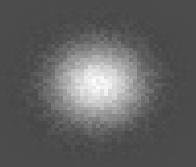
\includegraphics[width=0.25\textwidth,height=0.25\textwidth]{figures/ch1_8_intermediateAsyn.jpeg} & 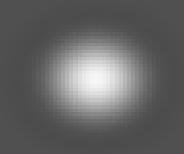
\includegraphics[width=0.25\textwidth,height=0.25\textwidth]{figures/ch1_8_finalAsyn.jpeg}\\
\hline
\end{tabular}
\end{center}

 \caption{Un exemple de traitement asynchrone des cartes neuronales (implémentation évènementielle), en appliquant les critères de convergence dérivés ici. Nous avons vérifié numériquement la conjecture que les résultats actuels s'appliquent lorsque l'évaluation est asynchrone. {\em Vue gauche}: résultat intermédiaire, la randomisation est visible. {\em Vue droite}: résultat final, après la convergence. Cela a été expérimenté sur un DNF $ 128 \times 128 $ avec un profil de connectivité latérale en différence de Gaussiennes, en utilisant les mêmes valeurs dans les cas synchrones et asynchrones. Deux paradigmes asynchrones ont été expérimentées: (1) En utilisant les temps de mise à jour aléatoires uniformément établis dans un intervalle compatible avec les conditions de Mitra. (2) Un mécanisme ``parcimonieux'' , voir le texte pour plus de détails.}

\label{fig: bump} 
\end{figure}

Ici les dates de mises à jour $ \Delta_ {ij} $ ont diminué comme une fonction linéaire de la variabilité de la valeur de l'état ​​$ \Delta V_i$ (mise à jour rapide pour les valeurs qui varient rapidement),
et nous avons simplement choisi $ \Delta_{ij} = \Delta_{max } \, (1 - \Delta V_i / \Delta V_ {max}) $, pour obtenir des retards entre $ 1$ et $ 10 $ périodes d'échantillonnage. Cela a considérablement diminué le nombre d'étapes (mieux que dans le paradigme synchrone), une étude précise sera une perspective de ce travail.\\

\section{Discussion}


Dans ce chapitre nous avons examiné les quatre aspects importants du cadre de modélisation:
\begin{enumerate}
\item Le neurone comme unité de base et règle de calcul locale.
\item L'approche connexionniste et la plasticité synaptique.
\item L'intégration numérique et les problèmes de discrétisation dans le cadre particulier de la CNFT, en particulier l'étude du biais entre une trajectoire continue et son approximation discrétisée au cours du temps.
\item L'utilisation de mécanismes synchrones/asynchrones à la fois au niveau de la modélisation et au niveau de l'implémentation dans une approche de calcul distribué, en particulier les garanties de convergence de l'évaluation asynchrone vers la solution prévue.\\
\end{enumerate}

Nous nous sommes concentrés sur le 3{\ieme} et le 4{\ieme} point en nous plaçant dans le cadre des DNF. Nous avons montré que des méthodes d'évaluation asynchrones peuvent être efficacement utilisées pour la simulation dynamique des champs de neurones. Dès que des hypothèses raisonnables sont vérifiées, la convergence rapide et la faiblesse du biais sont garantis. En retour, comme nous l'avons expliqué dans la section \ref{convergence}, la théorie des champs de neurones dynamiques fournit un bon terrain pour l'étude des systèmes d'évaluation asynchrone. Par exemple, dans \cite {Rougier:2006}, il a été démontré (numériquement) que cette méthode d'évaluation asynchrone conduit à de nouvelles solutions stables qui sont fonctionnellement différentes de celles obtenues par le schéma continu. Lorsqu'on présente deux stimuli identiques à deux endroits différents, le champ est capable de se stabiliser sur l'un ou l'autre des deux stimuli et donc briser la symétrie du système. Toutefois, on peut montrer facilement que ce nouvel état très stable peut ne pas être une solution de l'équation continue du champ. Quel est donc la pertinence d'une telle description continue si l'on veut l'évaluer en utilisant les équations numériques asynchrones? Idéalement, nous aimerions pouvoir disposer d'une description asynchrone continue équivalente mais malheureusement, ce n'est pas encore le cas dans le domaine des mathématiques. Nous devrions alors prendre des précautions supplémentaires lors de la description d'un système décrit par des équations continues et la question suivante se pose : est ce qu'on simule vraiment ce que nous avons annoncé dans la définition du système? En particulier, au niveau de la modélisation mésoscopique, il peut être intéressant d'utiliser un paradigme basé sur les événements au lieu d'une horloge centrale, car il s'agit d'un paradigme qui prend en considération le fait que non seulement le traitement mais aussi le calendrier de mises à jour sont entièrement distribués. \\

D'un point de vue plus cognitif, cette étude révèle la présence implicite d'une horloge centrale dans un certain nombre de modèles et donc la présence implicite d'un grand superviseur pour orchestrer l'activité globale du modèle. Une future étape du travail sera l'utilisation d'un cadre basé sur le codage événementiel où il est possible de contrôler, à la fois, la valeur et le {\em temps} de mise à jour de cette valeur. Il est possible de simuler dans un tel cadre tous les régimes asynchrones possibles (schéma périodique, relaxation chaotique, etc. \cite {Chazan:1969, Amitai:1993}). Une telle plate-forme permet donc de déterminer quel schéma numérique asynchrone est pertinent pour une modélisation temporelle donnée, ouvrant la voie pour étudier concrètement au niveau mésoscopique, le temps de calcul. En fait, si les limites examinées dans le présent document garantissent la convergence, rien ne peut a priori être déclaré sur les performances, ou l'émergence de phénomènes transitoires, etc.\\

Enfin, l'évaluation asynchrone a l'avantage d'être un schéma de calcul qui s'approche plus de la réalité du système nerveux qui s'articule autour d'unités élémentaires indépendantes. En plus, ce paradigme est en faveur de l'implémentation informatique distribuée fortement souhaitée d'un point de vue informatique. Mais comme on peut le constater dans ce chapitre, la mise en oeuvre d'un tel schéma de calcul rend à la fois la modélisation et l'implémentation plus compliquées. C'est pourquoi nous avons choisi le schéma d'évaluation synchrone dans les modèles que nous allons proposer par la suite puisqu'on va se concentrer plus sur les flux d'information et les propriétés émergentes des dynamiques locales. De plus, puisqu'on se place à l'échelle mésoscopique en s'intéressant à la modélisation des structures corticales et sous-corticales nous avons adopté le codage fréquentiel. Le codage impulsionnel étant plus adapté à la modélisation à l'échelle du neurone, l'utiliser pour des modèles d'interactions de plusieurs populations de neurones nécessite plus de puissance de calcul. De plus si les propriétés temporelles des trains de spikes (dates, phases, synchronie...) ne sont pas examinées et seule la fréquence moyenne de décharge est évaluée, il n'est pas nécessaire de passer par une modélisation à spikes. Enfin, tous les mécanismes présentés dans nos modèles ont été simulés en utilisant la méthode d'Euler qui est la moins coûteuse en termes de calcul et la plus simple. En utilisant cette méthode, nous avons conscience des erreurs de simulation par rapport au système à temps continu et nous optons pour des temps d'échantillonnage faibles permettant de conserver les propriétés émergentes des interactions.


